%%%%%%%%%%%%%%%%%%%%%%%%%%%%%%%%%%%%%%%%%%%%%%%%%%%%%%%%%%%
% EPFL report package, main thesis file
% Goal: provide formatting for theses and project reports
% Author: Mathias Payer <mathias.payer@epfl.ch>
%
% This work may be distributed and/or modified under the
% conditions of the LaTeX Project Public License, either version 1.3
% of this license or (at your option) any later version.
% The latest version of this license is in
%   http://www.latex-project.org/lppl.txt
%
%%%%%%%%%%%%%%%%%%%%%%%%%%%%%%%%%%%%%%%%%%%%%%%%%%%%%%%%%%%
\documentclass[a4paper,11pt,oneside]{report}
% Options: MScThesis, BScThesis, MScProject, BScProject
\usepackage[MScThesis,lablogo]{EPFLreport}
\usepackage{datetime}
\usepackage{amsmath}
\usepackage{amssymb}
\usepackage{xspace}
\usepackage{array}
\usepackage{lscape}
\usepackage{booktabs}
\usepackage{subcaption}
\usepackage{gensymb}
\usepackage{stmaryrd}
\usepackage{verbatim}
\usepackage{siunitx}
\usepackage{algpseudocode}
\usepackage{algorithm}


\usepackage{hyperref}
\usepackage{graphicx}

\title{Regional Climate Model Emulator based on Deep Learning: SMB predictions over Antarctica}
\author{Marijn van der Meer}
\supervisor{Sophie de Roda Husman}
\adviser{Prof. Dr. sc. EPFL Martin Jäggi}
\expert{Prof. Dr. sc. TU Delft Stef Lhermitte}

\newcommand{\sysname}{FooSystem\xspace}

\begin{document}
\maketitle
\makededication
\makeacks

\begin{abstract}
The \sysname tool enables lateral decomposition of a multi-dimensional
flux compensator along the timing and space axes.

The abstract serves as an executive summary of your project.
Your abstract should cover at least the following topics, 1-2 sentences for
each: what area you are in, the problem you focus on, why existing work is
insufficient, what the high-level intuition of your work is, maybe a neat
design or implementation decision, and key results of your evaluation.
\end{abstract}

\begin{frenchabstract}
For a doctoral thesis, you have to provide a French translation of the
English abstract. For other projects this is optional.
\end{frenchabstract}

\maketoc

%%%%%%%%%%%%%%%%%%%%%%
\chapter{Introduction}
%%%%%%%%%%%%%%%%%%%%%%

\textbf{Flow of introduction section}:
\begin{itemize}
    \item Par 0: short summary of project
    \item Par 1: discuss the setting
    \item Par 2: introduce the main challenge that you see
    \item Par 3: lists why related work is insufficient
    \item Par 4-5: discuss your approach and why it is needed
    \item Par 6: introduce your thesis statement
    \item Par 7: highlight some of your results
    \item Par 8: discusses your core contribution
\end{itemize}
 
 
\begin{itemize}
    
    \item \textbf{Paragraph 0} - Short summary of project: This thesis aimed to develop a machine learning framework that learns the downscaling function of regional climate models. Specifically, we wanted to emulate i.e., imitate, regional surface mass balance values of the Antarctic ice sheet on the Antarctic Peninsula. We wanted to create a machine learning model that inputs low-resolution climate variables and outputs a high-resolution surface mass balance map. Note here that by low-resolution, we mean coarse images; with high resolution, we mean fine images. We got inspired for our framework by a paper by a Meteo France group that used machine learning to emulate regional near-surface temperature over western Europe~\cite{Doury}.
    \item \textbf{Paragraph 1}-Discuss the setting: Antarctic ice sheet and SMB. Why is it important?
    \begin{itemize}
        \item AIS: The Antarctic ice sheet (AIS) is the largest class of glaciers and contains the majority of ice on Earth, with a volume of 30 million cubic kilometers~\cite{Icesheetsquick}. It extends over 14 million square kilometers, roughly the combined area of the US and Mexico~\cite{AntarcticIceSheet}. This amount of ice constantly changes through melting processes and with the addition of new mass from snow and ice.
        \item SMB: A primary variable used to observe the AIS is surface mass balance (SMB). SMB is the net balance between inputs and outputs of mass (of ice and snow) on top of the ice sheet~\cite{Lenaerts}. It is influenced by the addition of mass through precipitation and snow‐transporting winds and ablation via erosion, sublimation, and run-off~\cite{Kittel}. At any point, an SMB close to zero indicates an arid climate with little change in the ice mass, while a positive SMB means that there was a lot of addition of mass, through precipitation, for example. On the other hand, a negative SMB means that a glacier is losing mass. In the case of ice sheets and grounded glaciers, this mass loss directly affects sea-level rise~\cite{icesheet}. 
        
        If Antarctica's ice sheet were to melt suddenly, sea levels would rise to approximately $60$\si{m}~\cite{Kittel, Fretwell, Morlighem}, making the AIS the most significant potential contributor to sea-level rise. Unfortunately, the AIS has been steadily losing mass since 2002~\cite{Shepherd, Mottram}, mainly because of calving\footnote{Calving is the process of chunks of ice breaking off from the edge of a glacier~\cite{Marshak}} and melting at the water-ice interface underneath ice shelves (submarine melting)~\cite{Kittel, Mottram, Rignot}. Because the SMB is a good indicator of stability and evolution of ice shelves, it is therefore imperative to have a precise estimation of the SMB of the AIS~\cite{icesheet}.
    \end{itemize}
    \item \textbf{Paragraph 2} - Can introduce the main challenge that you see: modelling SMB is very difficult. Done mainly with climate simulations but computationally expensive. 
    \begin{itemize}
        \item Though SMB can be monitored with on-site tools, in this project, we used data from satellite remote sensing data. 
        \item To understand and predict the behaviour of different climate phenomena, climatologists have come up with complex climate models, which are simulations of climate variables over time and space in different parts of the world. 
        \item At our current technological level, the complexity of these climate models is a compromise between computational costs, resolution of pixels and the width of region that is covered. 
        \item Depending on the spatial resolution we want, we usually define two types of climate models: global climate models (GCM) and regional models (RCM). 
    \end{itemize}
    \item third paragraph lists why related work is insufficient: emulator done for temperature but not for SMB over Antarctica
    \item fourth and fifth paragraphs discuss your approach and why it is needed: emulator from doury extended to smb
    \item sixth paragraph will introduce your thesis statement. Think how you can distill the essence of your thesis into a single sentence.
    \item The seventh paragraph will highlight some of your results
    \item The eights paragraph discusses your core contribution.

\end{itemize}


\begin{itemize}
    \item Traditional U-Net is a fully convolutional CNN architecture specifically developed for biomedical image segmentation~\cite{Ronneberger2015}.  
        \item U-Net shows high performance in classification and segmentation tasks where the network is trained to predict a class for each pixel. But U-Nets are also used for image processing tasks, such as super resolution. They have been found to be particularly effective in cases where the output and inputs are of similar size. In our case, we applied it to a time series prediction task in which the network has to predict an exact value for each pixel.
    \item using attention in a CNN facilitates the network to focus on specific parts of the input. 
\end{itemize}

Surface mass balance (SMB) provides mass input to the surface of the Antarctic and Greenland Ice Sheets and therefore comprises an important control on ice sheet mass balance and resulting contribution to global sea level change. As ice sheet SMB varies highly across multiple scales of space (meters to hundreds of kilometers) and time (hourly to decadal), it is notoriously challenging to observe and represent in models. In addition, SMB consists of multiple components, all of which depend on complex interactions between the atmosphere and the snow/ice surface, large-scale atmospheric circulation and ocean conditions, and ice sheet topography.~\cite{Lenaerts}


\section{Regional Climate Model Emulator based on Deep Learning: Concept and First Evaluation of a Novel Hybrid Downscaling Approach \cite{Doury}}
This paper proposes a novel hybrid downscaling approach that emulates the downscaling function of a a regional climate model.

\begin{itemize}
\item RCM: EURO-CORDEX simulations based on the CNRM-ALADIN63, 1951-2100 RCP4.5 and RCP8.5
\item GCM: CNRM-CM5 used in CMIP5 → 6h frequency + sea surface temperature, sea ice cover and aerosol optical depth at monthly frequency
\item ML model learns the RCM transformation of the large-scale climate information into local-scale
\item Target variable: near surface temperature (TAS)
\item Target domain: southwest European domain
\item Historical period: 1951 to 2005
\item Scenarios (2006-2100): based on two Representative Concentration Pathways from CMIP5; RCP4.5 and RCP8.5
\end{itemize}
Computational performance:
\begin{itemize}
    \item U-Net: fully convolutional neural network algorithm
    \item Substantial computational gain regarding RCM computational cost
    \begin{itemize}
        \item 2h training on GPU + downscaling instantaneous
        \item RCM simulation involves weeks of computation on super-computer
    \end{itemize}
\end{itemize}
Training of model 
\begin{itemize}
    \item RCM can be broken down into a large scale transformation and a downscaling function
    \item Training using existing RCM simulations → learn large scale/local scale relationship in different climates and in future climate
    \item Training in perfect model framework: input and output to ML model come from same RCM simulation → focus on downscaling function
    \item Input variable: daily large-scale and low-resolution RCM information (upsampled to GCM like resolution)
    \item Output variable: daily maps of TAS at RCM resolution (~12 \si{mmWe/day}\sci{km})
    \item Emulator is RCM-dependent as downscaling function depends on RCM choice
\end{itemize}
Results
\begin{itemize}
    \item Emulator evaluated in both perfect model (evaluation 1) and GCM worlds (evaluation 2)
    \item capture very well transformation from low resolution information to high resolution TAS
    \item robust to different sources of input
    \item succeeds very well in reproducing high resolution spatial structure and daily variability of the RCM
    \item evaluation 1 shows that emulator is able to reproduce original series almost perfectly
    \item training emulator in future climate improves its ability to reproduce warmer climate
    \item limitations in accurately simulating extreme events and complete climate change magnitude
    \item RCM-GCM large scales inconsistencies when evaluating on GCM. Does not learn to reproduce large scale transformations (because trained only on RCM)
\end{itemize}
\section{Diverging future surface mass balance between the Antarctic ice shelves and grounded ice sheet \cite{Kittel}}

\section{SmaAt-UNet: Precipitation Nowcasting using a Small Attention-UNet Architecture~\cite{smatunet}}



%%%%%%%%%%%%%%%%
\chapter{Model and methods}
%%%%%%%%%%%%%%%%

\begin{table}[!tbp]
    \centering
    \caption{}
    \renewcommand\arraystretch{1.5}
    \begin{tabular}{l>{\raggedright\arraybackslash}p{0.4\linewidth}>{\raggedright\arraybackslash}p{0.4\linewidth}}
    \toprule
        \textbf{Notation} & \textbf{Description} & \textbf{Dimensions} \\ \toprule 
        $\mathcal{D}$ & Input Domain & $\llbracket 1, I \rrbracket \times \llbracket 1, J \rrbracket$   \\
        $\mathcal{E}$ & Target Domain & $\llbracket 1, K \rrbracket \times \llbracket 1, L \rrbracket$   \\
        $(i,j)$ & Spatial indexes over
        input grid & $\mathcal{D}$   \\
        $(k,l)$ & Spatial indexes over
        target grid & $\mathcal{E}$   \\
        $X$ & Input: set of 2D variables over $\mathcal{D}$ & $T \times \llbracket 1, I \rrbracket \times \llbracket 1, J \rrbracket \times C_1$   \\
        $Z$ & Input: set of 1D variables over $\mathcal{D}$ & $T \times C_2$   \\
        $Y$ & Target: surface mass balance over $\mathcal{E}$ & $T \times \llbracket 1, K \rrbracket \times \llbracket 1, L \rrbracket$  \\
        $t$ & Monthly temporal index & $T$   \\
        $x$ & 2D variables index & $C_1$   \\
        $z$ & 1D variables index & $C_2$ 
        \\
        $F$ & Downscaling function of the RCM & 
        \\
        $\hat{F}$ & Emulator: Estimation of F & 
        \\
        $\operatorname{UPRCM}$ & GCM-like: upscaled RCM to GCM resolution & 
        \\
\bottomrule
    \end{tabular}
        \subcaption*{\small Table~\ref{tab:notations}. Notations used in this paper.}
            \label{tab:notations}
\end{table}

\begin{itemize}
\item \textbf{Global idea}: we built an RCM-emulator $\hat{F}$ that uses a neural network architecture to estimate the downscaling function $F$ in 
\begin{equation}\label{eq:emulator-equation}
    Y = \operatorname{F}(X) \;\;\;\; X\subset\mathcal{D}, Y\subset\mathcal{E}
    \end{equation}
where $X$ are low-resolution variables from a global climate simulation over an input domain $\mathcal{D}$ and $Y$ is a high-resolution surface variable of a regional climate model over a target domain $\mathcal{E}$. 
\item Flow of model and methods section: 
\begin{itemize}
    \item Data: climate models used -> target and input domains -> variables chosen (input features for model)
    \item Model: architecture -> perfect model framework (creation of UPRCM) -> training flow (on GCM and UPRCM) -> evaluation process
\end{itemize}
\end{itemize}

\section{Data}\label{sec:data}
\subsection{Climate model}
\begin{itemize}
   \item RCM: RCM variable emulated by $\hat{F}$ is the daily surface mass balance (SMB) values from MAR(ACCESS1.3), a regional downscaling of the global climate model ACCESS 1.3 (CMIP5~\cite{ACCESS13, CMIP5}) by the Modèle Atmosphérique Régional (MAR). 
    \item MAR is known for accurately modeling physical processes in polar regions such as surface mass balance, air-snow interactions, and atmospheric circulation over ice sheets~\cite{MAR}. 
    \item Why: According to studies comparing climate models conducted in~\cite{Kittel, Agosta2015}, ACCESS 1.3 and MAR(ACCESS 1.3) were the models that most accurately represented the present Antarctic climate in comparison to ERA-Interim. For this reason, we chose MAR(ACCESS 1.3) and its corresponding global climate model as climate simulations for our Emulator.  
    \item Time-frame: historical values from 1980-2006 and future climate simulation RCP 8.5~\cite{Moss2010} from 2006-2100. 
    \item Grid and resolution: the RCM grid is in south polar stereographic coordinates of $35 \times 35$ \si{km} resolution. The GCM resolution is of 1.25° latitude by 1.875° longitude (approximately $68 \times 206$ \si{km}), using a staggered Arakawa C grid~\cite{ACCESS13, ACCESS13_2}. 
    \item Reprojection: So that both regional and global climate models are in the same projection system, we project the GCM to south polar stereographic coordinates (see Annex for details~\ref{sec:preproc-GCM}). 
\end{itemize}

\begin{figure}[!t]
  \centering
  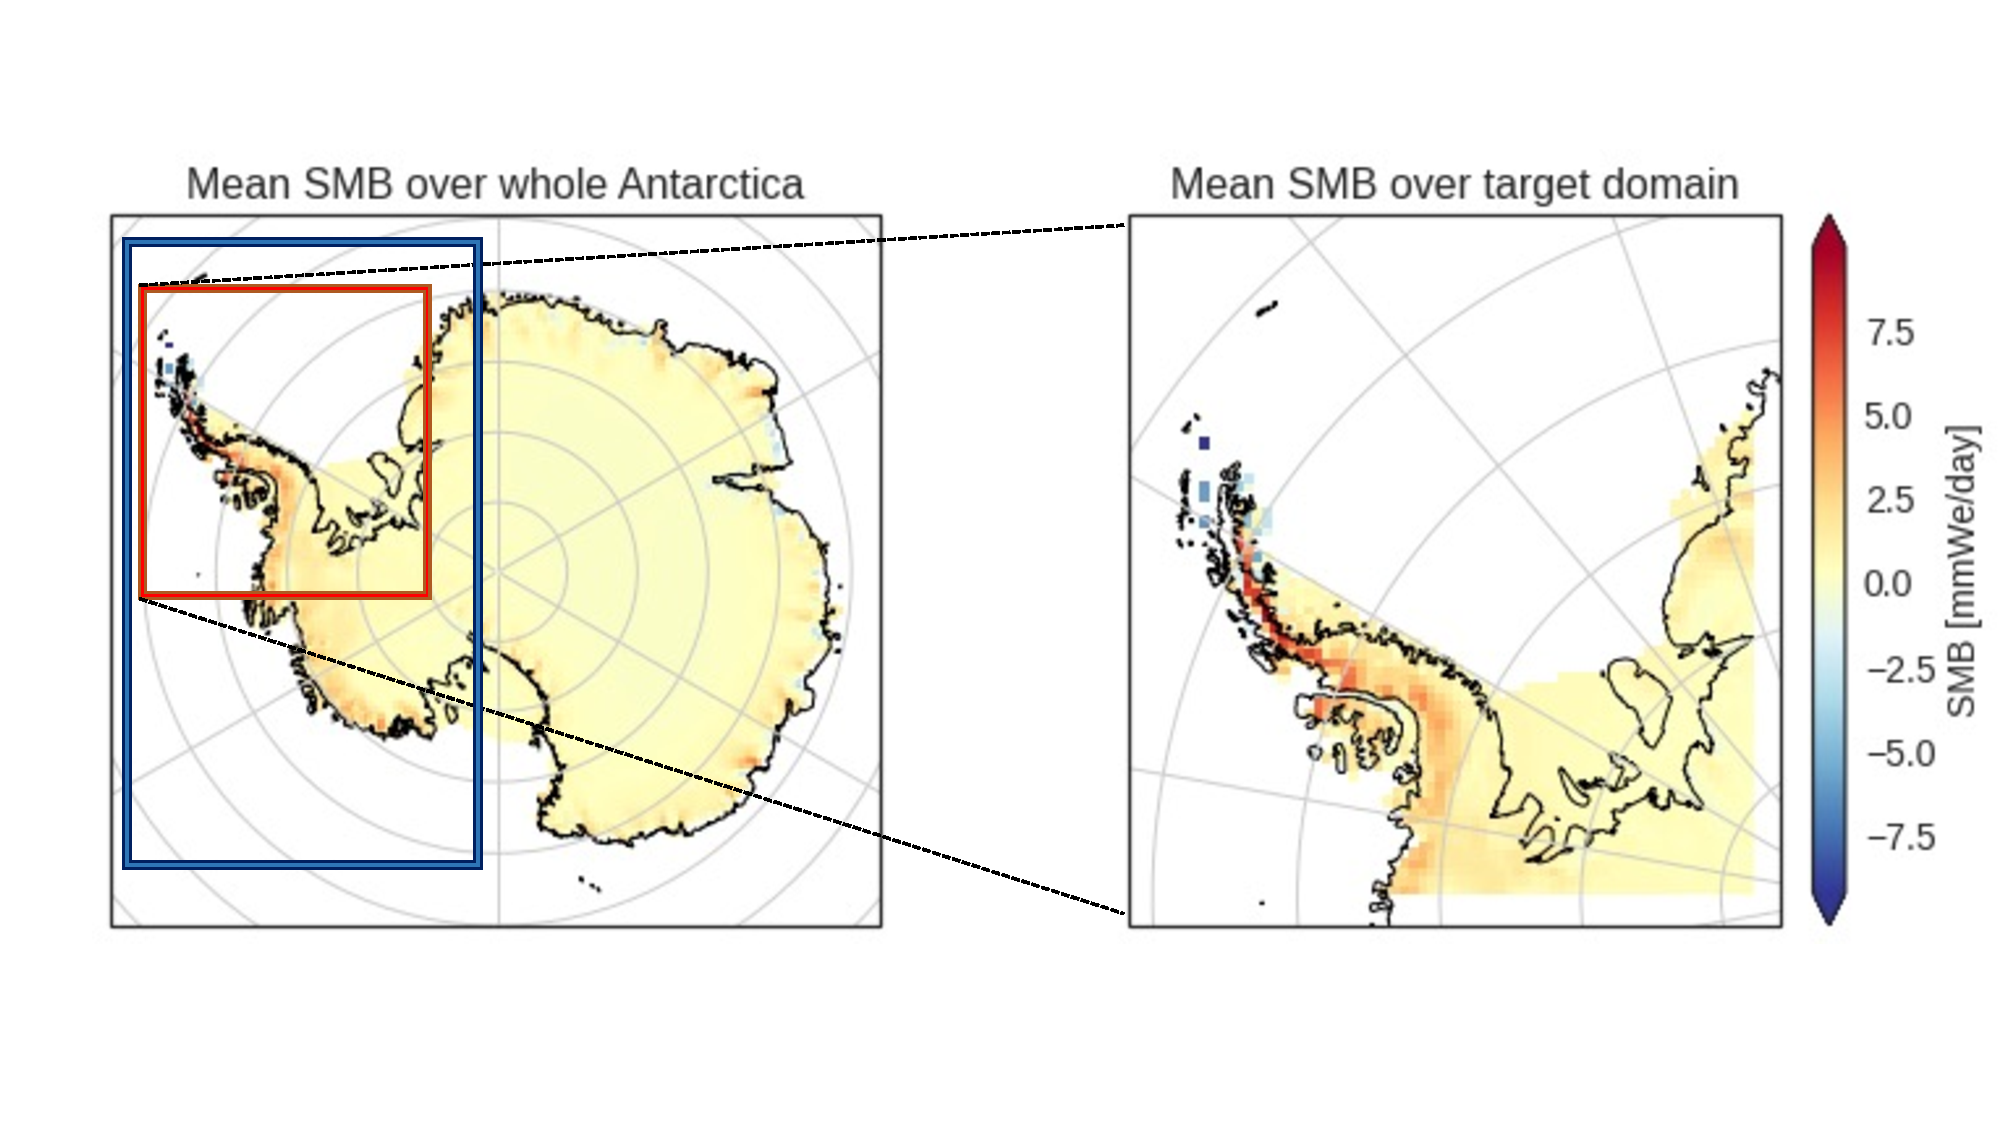
\includegraphics[width=\columnwidth]{images/domains.pdf}
  \caption []{\small Daily mean surface mass balance over Antarctica (left) and the Antarctic Peninsula (right) from 1990-2100. Regions chosen as target domain $\mathcal{E}$ (in red) and input domain $\mathcal{D}$ (in blue) for the Emulator.}
  \vspace{-3mm}
    \label{fig:region-of-choice}
\end{figure}


\subsection{Target and input domain}
\begin{itemize}
   \item Target domain: The target domain used for this model is a grid box of $64 \times 64$ pixels at $35$ \si{km} resolution that contains the Antarctic Peninsula in West Antarctica. 
    \item Antarctic Peninsula: 
    \begin{itemize}
        \item The Antarctic Peninsula is the most northern part of Antarctica
        \item It covers approximately 5 million square kilometers and is mainly covered by ice. Major ice shelves include the Larsen and Ronne ice shelves.
        \item It is very mountainous, with its highest peaks rising to about $3'000$ \si{m}
        \item Temperature: the Peninsula has the mildest climates on this continent. Its temperatures are warmest in January, averaging $2$ $\degree C$, and coldest in June, averaging from $-15$ to $-20$ $\degree C$~\cite{AntarcticPeninsula}
        \item Precipitation: Precipitation varies significantly within the Antarctic Peninsula. The peninsula's tip has the highest precipitation levels, with $35-50$ \si{cm} per year. On the west coast and northeast coast, occasional rain leaves precipitation at $35$ \si{cm}. Along the east coast and the interior of Antarctica, the climate is drier, with precipitation that ranges from $10-15$ \si{cm}~\cite{antarctic-climate, antarctic-climate-2}
    \end{itemize} 
    \item Why this target region: 
    \begin{itemize}
        \item Because of the specific patterns of climate variables such as temperature and precipitation, the Antarctic Peninsula has a high annual and geographical variability in SMB values. 
        \item This shows when looking at mean SMB values as in Fig.~\ref{fig:region-of-choice}. The Peninsula's tip and west coast offer higher values than the rest. Mean SMB values range from approximately $-10$ to $10$ \si{mmWe/day} while the extremes observed in this region from 1980 to 2100 are a minimum of $-59$ \si{mmWe/day} and a maximum of $30$ \si{mmWe/day}. 
        \item All of this makes this region very interesting to us because we want to see how the Emulator adapts to different annual patterns of SMB over our target domain.  
    \end{itemize}
    \item Input domain: the input domain is a $48\times25$ grid box at ($68 \times 206$ \si{km} resolution) (Fig.~\ref{fig:region-of-choice}) defined around the target domain. It covers approximately 17 million square kilometers. Because it is favorable to give our machine learning model a square input, it is resized to $32\times 32$ by bilinear interpolation. 
\end{itemize}


\subsection{Features}\label{subsec:features}
\begin{itemize}
    \item The Emulator receives as input features $(X, Z)$ that consist of two-dimensional variable $X$, and one-dimensional $Z$ (Table~\ref{tab:features}). 
    \item Spatial encoding X:
    \begin{itemize}
        \item The two-dimensional feature $X$ contains eight different atmospheric variables measured daily at (near) surface level. After a monthly mean aggregation, the frequency of variables is monthly.
         \item Normalisation of X: These variables are normalised according to their spatial mean $\bar{X}_{t,x}$ and standard deviation $\sigma(X_{t,x})$ for each time-step $t\in T$:
            \begin{equation}\label{eq:normalisation-X}
            \tilde{X}_{t,i,j,x} = \frac{X_{t,i,j,x}-\bar{X}_{t,x}}{\sigma(X_{t,x})} \;\;\;\; t\in T, \forall (i,j) \in \mathcal{D}, x\in C_1
        \end{equation}
        \item Feature selection: In terms of feature selection, we decided to follow the same procedure as in~\cite{Doury} and give all available variables to the Emulator. 
        \begin{comment}
        and later evaluate their feature importance. 
        \end{comment}
    \end{itemize}
\item Temporal encoding Z: \begin{itemize}
    \item 
The one-dimensional variable $Z$ includes the time-series of spatial means $\bar{X}_{t,x}$ and standard deviations $\sigma(X_{t,x})$ for each atmospheric variable $x\in C_1$ and time step $t\in T$.

\item It also includes a cosine, sine vector to encode the information about the month of the year.
    \begin{equation*}
       \operatorname{cos}\left(\frac{2\pi t}{12}\right);\; \operatorname{sin}\left(\frac{2\pi t}{12}\right) \;\;\;\; \forall t\in T
    \end{equation*}
    
    \item Overall this gives the following equation for $Z$:
    \begin{equation}\label{eq:Z}
    Z = \left[ \bar{X}_{t\in T, x\in C_1}, \sigma\left(X_{t\in T, x\in C_1}\right), \operatorname{cos}, \operatorname{sin} \right] \subset T \times C_2
\end{equation}
    \item Why?: because the $X$ variables are normalized at each time step by their spatial mean, they do not carry any temporal encoding. Adding Z to the model allows it to have access to this information. 
\item Normalisation of Z: each of the spatial means $\bar{X}_{t,x}$ and standard deviations $\sigma(X_{t,x})$ in Z are normalised according to a reference period ($\mathrm{ref}=$1980-2000)~\cite{Doury}:
\begin{equation}\label{eq:normalisation-Z}
    \tilde{Z}_{t,z} = \frac{Z_{t,z}-\bar{Z}_{\mathrm{\mathrm{ref}},z}}{\sigma(Z_{\mathrm{ref},z})} \;\;\;\; t\in T, z\in C_2
\end{equation}
where $\bar{Z}_{\mathrm{ref},z}$ and $\sigma(Z_{\mathrm{ref},z})$ are respectively the temporal mean and standard deviation of the spatial means or standard deviations of $X_{\mathrm{ref}, x} \subset T_{\mathrm{ref}}\times C_1$.
\end{itemize}



\end{itemize}

\begin{table}[tbp]
    \centering
    \caption{}
    \renewcommand\arraystretch{1.5}
    \begin{tabular}{l>{\centering}p{0.1\linewidth}>{\centering}p{0.2\linewidth}>{\centering\arraybackslash}p{0.2\linewidth}}
    \toprule
        \textbf{Variable Name} & \textbf{Variable Notation} & \textbf{Units} & \textbf{Dimensions} \\ \toprule
        \textbf{2D variables} & & & \\ \bottomrule 
        Northward Wind & NW & $[ms^-1]$ & $ \mathcal{D}$   \\ 
        Eastward Wind & EW & $[ms^-1]$ & $ \mathcal{D}$ \\
        Downwelling Shortwave Radiation & SWD & $[Wm^{-2}]$ & $ \mathcal{D}$ \\
        Downwelling Longwave Radiation & LWD & $[Wm^{-2}]$ & $ \mathcal{D}$ \\
        Specific Humidity & QQP & $[g/Kg]$ & $ \mathcal{D}$ \\
        Temperature & TT & $[\degree]$ & $ \mathcal{D}$ \\
        Precipitation & PR & $[mmWe/day]$ & $ \mathcal{D}$  \\
        Pressure & PR & $[hPa]$ & $ \mathcal{D}$  \\
        \toprule
         \textbf{1D variables} & & & \\ \bottomrule
        Spatial mean of 2D variables & $\bar{X}_{x}$ & & $[C_1]$ \\ 
        Spatial std of 2D variables & $\sigma\left(X_{x}\right)$ & & $[C_2]$ \\
        Seasonal Indicators & & & $[2]$\\ \bottomrule
        
    \end{tabular}
        \subcaption*{\small Table~\ref{tab:features}. Two and one-dimensional input features given to the model. Each feature is measured (near) surface and a monthly mean aggregation.}
            \label{tab:features}
\end{table}


\section{Model}\label{sec:model}

\begin{figure}[!t]
  \centering
  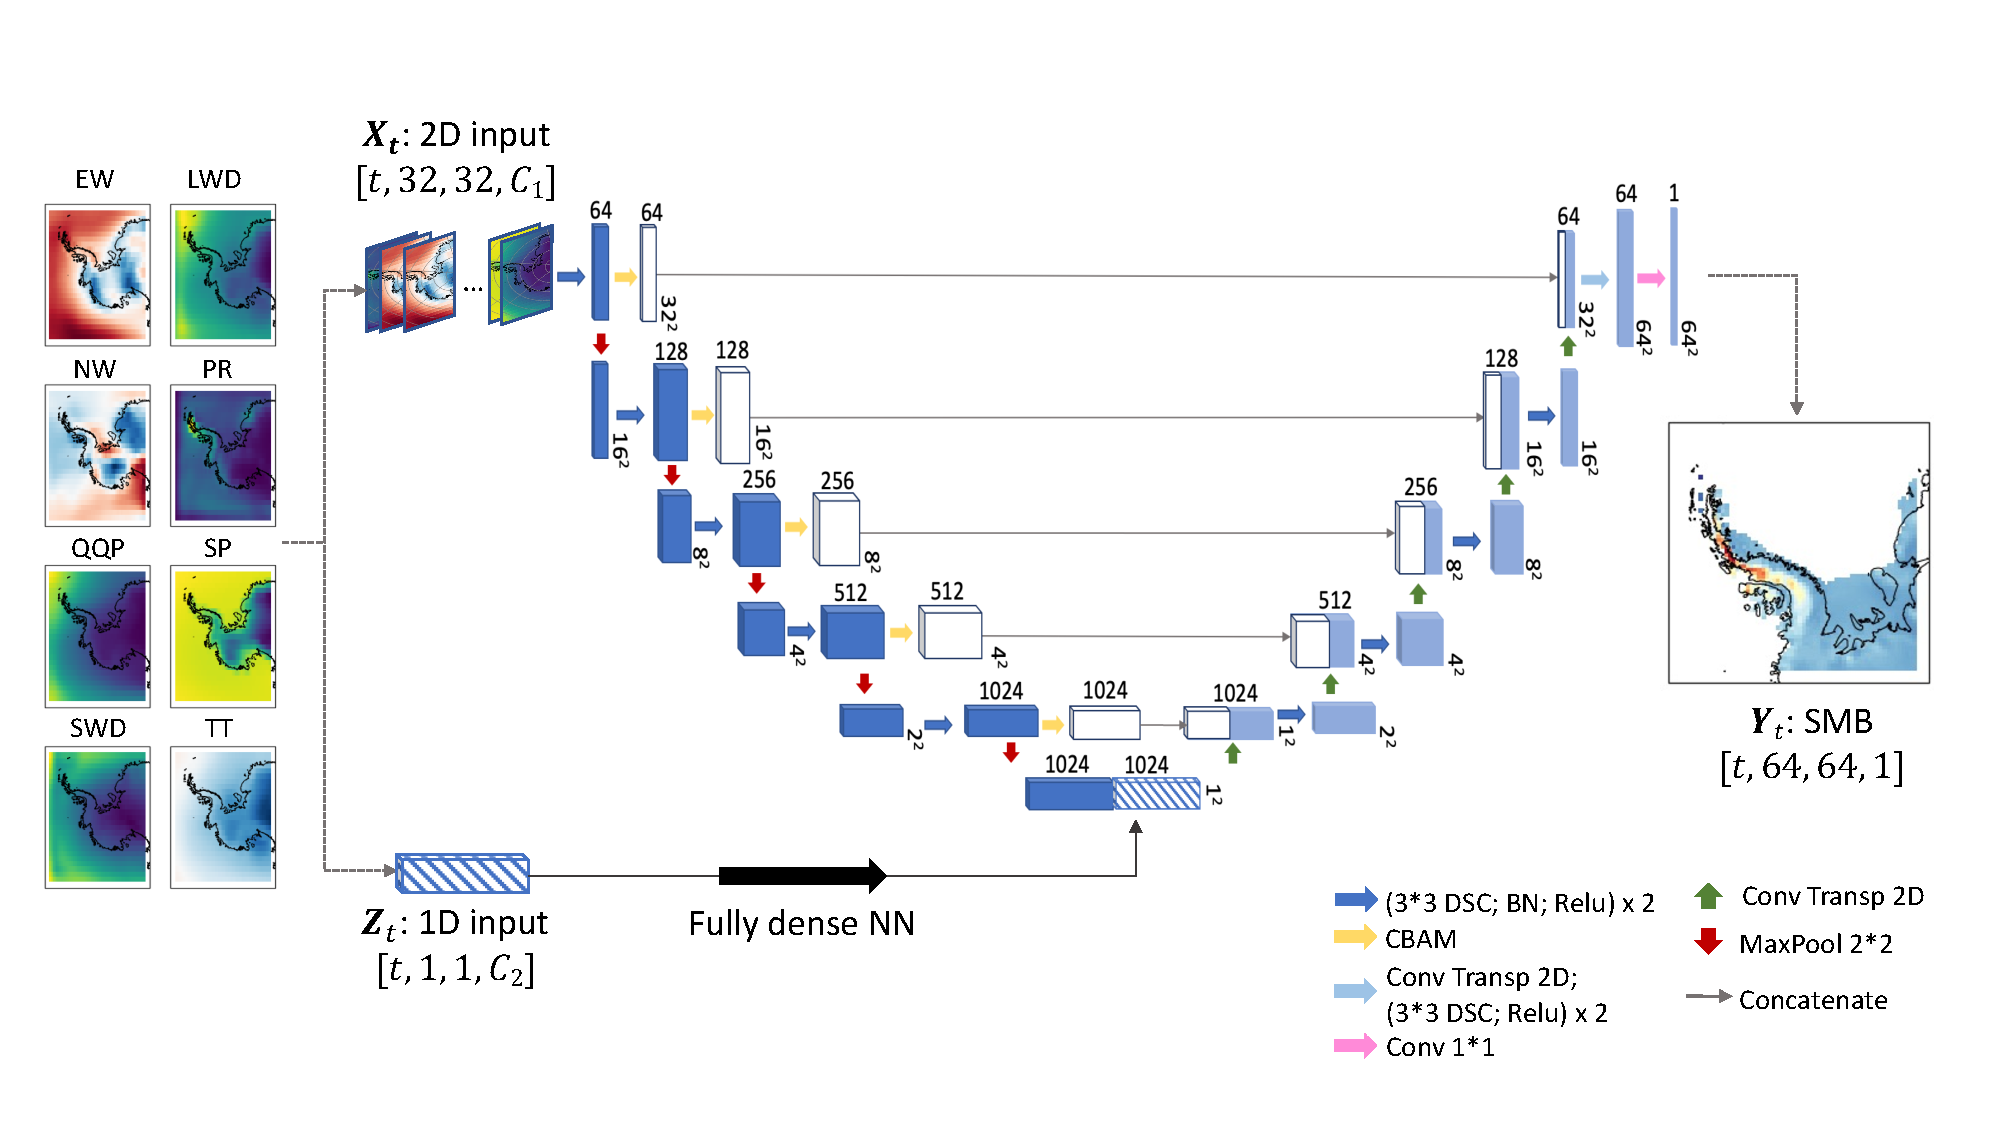
\includegraphics[width=\columnwidth]{doc/Thesis-latex/images/unet-with-data.pdf}
  \caption []{\small Illustration of an observation at time-step $t$. Left: 2D input variables $X_t$ on the input domain with its corresponding 1D variable $Z_t$. Right: target surface mass balance (SMB) $Y_t$ on the target domain. Middle: scheme of the U-Net architecture used for this paper. }
  \vspace{-3mm}
  \label{fig:example-features}
\end{figure}

\subsection{Architecture}\label{subsec:architecture}
\begin{itemize}
    \item The Emulator's architecture extends the U-Net used to emulate near-surface temperature in~\cite{Doury} with mechanisms from the SmaAt-UNet model~\cite{smatunet} (Fig.~\ref{fig:example-features}).
     \item SmaAt-UNet: SmaAt-UNet extends the traditional U-Net architecture~\cite{unet} with CBAM attention mechanism and depthwise-separable convolutions instead of regular convolutional operations. 
    \item Architecture: 
    \begin{itemize}
    \item The network is U-shaped as it is divided into a down-sampling/encoder section that forms the left side and an up-sampling/decoder on the right.
    \item Encoder: the Encoder consists of double convolution (blue arrows) followed by max-pooling (red arrows). This process halves the image size and doubles the number of channels. Instead of the traditional U-Net convolutional operations, the Emulator uses depthwise-separable convolutions (DSC), designed to reduce the number of parameters~\cite{smatunet}.
    \item Bottom of U-Net: At the bottom of the U-Net, encoded spatial information from $X_t$ and temporal information from $Z_t$ are concatenated. The corresponding 1D input $Z_t$ of $X_t$ first goes through a fully dense neural network to reach the same number of channels as the output of the last layer of the Encoder. Then, it is concatenated with the Encoder output at the bottom of the “U”. This constrains the U-Net to give equal importance to the spatial and temporal inputs before starting the decoding path and generating the high-resolution SMB image~\cite{Doury}. 
    \item Decoder: three parts; a 2D transposed convolution operation (green arrows) to double the image size, a concatenation of the resulting feature maps with the previous Encoder’s attention maps (white blocks) via skip-connections (grey arrows), and lastly a double depthwise-separable to half the number of channels (blue arrows). 
    \item Skip-connections: skip-connections between layers (grey arrows) make it possible to skip large sections if required and create a smoother loss surface. 
    \item  Last layers: up-sampling layer (light blue arrow) to reach target size ($64\times 64$) and $1\times1$ convolution (pink arrow) to change the number of channels from $64$ to $1$, and outputs a single image representing the SMB values predicted by the network at time-step $t$.
    \item Attention: Convolutional block attention modules (CBAMs, yellow arrow)~\cite{smatunet} are placed after each double convolution in the Encoder and used to detect important features over the channels and spatial regions of the inputs. In CBAMs, the attention mechanism is first applied over the channels of the image and then the spatial dimension. Note that the input to the next layer of the Encoder is not the attention feature map (white block) but the convoluted and downsampled image of the previous layer (dark blue block). This way, the original image features are preserved throughout the Encoder layers. Finally, the attention blocks are fed through skip-connections to the corresponding Decoder layer to be concatenated~\cite{smatunet}. Contrary to the DSC convolutions used in the Encoder and Decoder, CBAMs use regular convolutions.  
    \end{itemize}
    \item Code: Architecture implemented in PyTorch 1.11 and available on \href{https://github.com/marvande/master-thesis}{GitHub}
\end{itemize}

\subsection{Perfect model framework}\label{subsec:perfect-model}
\begin{itemize}
    \item The authors of~\cite{Kittel} trained their Emulator in a \textit{perfect model framework} where both the low-resolution inputs and high-resolution SMB truth used in the Machine Learning model come from the same RCM simulation. 
    \item Why:
    \begin{itemize}
        \item Their Emulator aims to learn the downscaling function $F$ of the RCM in Eq.~\ref{eq:emulator-equation}.
        \item For this, the model needs perfect consistency (high temporal and spatial correlation) between the low-resolution inputs $X$ and the high-resolution target $Y$. Otherwise, the Emulator will try to learn a non-existing or non-exact relationship between $X$ and $Y$.
        \item Because of large-scale biases and inconsistencies between GCM and RCM variables, a perfect consistency cannot be guaranteed.
    \end{itemize}
    \item Creation of UPRCM: 
    \begin{itemize}
        \item To test the effect of this training framework on our Emulator, we followed the procedure outlined in~\cite{Doury} and create "GCM-like" features ($\operatorname{UPRCM}$).
        \item In a first step, we upscaled RCM features to GCM resolution ($68\times206$ km) through conservative interpolation. 
        \item In a second step, the upscaled RCM features were smoothed with a $3\times3$ moving average filter. This filter conserves the GCM grid, but each point now contains smoother information, and this further ensures the removal of local-scale information that might persist through the upscaling~\cite{Doury, Klaver2020}.
    \end{itemize}
    \item Consistency: To assess the presence of biases and inconsistencies between UPRCM and GCM features, we used two correlation statistics.  
    \begin{itemize}
        \item Temporal correlation: for each atmospheric variable $x\in C_1$ and point $p = (i,j)$ in the input domain $\mathcal{D}$, we calculated the Pearson correlation between the GCM and UPRCM time-series:
        \begin{equation}\label{eq:temporal-corr}
            \rho\left(G_{p}^x,U_{p}^x\right) = \frac{\operatorname{cov}(G_{p}^x,U_{p}^x)}{\sigma(G_{p}^x)\sigma(U_{p}^x)} \;\;\;\; \forall p \in \mathcal{D}, x\in C_1 
        \end{equation}
        where $G_{p}^x = \operatorname{GCM}[1:T, i, j, x]$, $U_{p}^x = \operatorname{UPRCM}[1:T, i, j, x]$, $\operatorname {cov}(\cdot)$  is the covariance and  $\sigma(\cdot)$ is the standard deviation.  
        \item Spatial correlation: for each $x\in C_1$ and time-step $t \in T$, we calculated the spatial correlation between GCM and UPRCM images: 
        \begin{equation}\label{eq:spatial-corr}
            \operatorname{sc}\left(G_{t}^x,U_{t}^x\right) = \frac{\operatorname{cov}(G_{t}^x,U_{t}^x)}{\sigma(G_{t}^x)\sigma(U_{t}^x)} \;\;\;\; \forall t \in T, x\in C_1 
        \end{equation}
        where $G_{t}^x = \operatorname{GCM}[t,1:I,1:J,x]$ and $U_{t}^x =\operatorname{UPRCM}[t,1:I,1:J,x]$. 
    \end{itemize}
\end{itemize}

\section{Training}\label{subsec:training}
\begin{itemize}
    \item Input to model: As aforementioned in~\ref{subsec:features}, each observation given to the Emulator are features $X_t$ and $Z_t$ for a month $t\in T$. $X_t$ is an array in $I \times J \times C_1$, where the two first dimensions are the spatial coordinates of the input domain, and the number of channels $C_1$ is the different atmospheric variables chosen as predictors. $Z_t \in C_2$ is its corresponding temporal encoding (Fig.~\ref{fig:example-features}).
    \item UPRCM and GCM: we created two Emulators by following two scenarios. We trained the first Emulator ($\operatorname{\hat{F}_U}$) following the perfect model framework (~\ref{subsec:perfect-model}) where we used upscaled RCM features as low-resolution inputs coming (UPRCM). Then, in a second step, we trained another Emulator ($\operatorname{\hat{F}_G}$) with coarse features directly from the GCM. 
    \item Why: The perfect model framework allowed us to evaluate how the U-Net performs when it has to learn only the downscaling function of the RCM. In the second training set, we wanted to see whether the model could learn the underlying dynamics, despite inconsistencies and biases, between GCM and RCM. 
    \item Loss: 
    \begin{itemize}
        \item In~\cite{Doury}, the authors propose to view the problem as regression and use Mean Squared Error (MSE) as a loss function. However, our Emulator performed poorly using an MSE loss and did not seem appropriate to our setting. 
        \item As aforementioned, the scale of SMB values vary significantly across the target domain. For example, dry inland points have minimal annual variations of SMB, with maximum values reaching under $2$ \si{mmWe/day}, while a point on the west coast can reach low extremes of $-20$ \si{mmWe/day}. In this unbalanced setting, MSE penalizes the ill-fitting of low SMB regions less than points with high values of SMB.  
        \item For this reason, we needed the points to be brought on the same scale when applying a loss function, so we chose to use a normalized RMSE (NRMSE) loss. Normalizing the RMSE facilitates comparing datasets with different scales, as in our case. 
        \item Equation: For each observation i.e., each time step $t$, given to the Emulator, we calculate the NRMSE loss between the predicted SMB value $\hat{Y}^{t}$ and the target $Y^{t}$ over all positions $p$ in the target domain $\mathcal{E}$:
        \begin{align}
        \operatorname{NRMSE}\left(Y^{t},\hat{Y}^{t}\right) &= \frac{RMSE}{Y_{\max} - Y_{\min}} \\
         &=\frac{\sqrt{\frac{1}{P}\sum_{p}(\hat{y}_{p}^{t}-y^{t}_{p})^2}}{Y_{\max} - Y_{\min}}   \;\;\;\; \forall t \in T
        \end{align}
        where $\hat{y}_{p}^{t}$ is the SMB value predicted at location $p\in \mathcal{E}$ and time $t \in T$, $P$ the number of points in $\mathcal{E}$ and $Y_{\max}$, $Y_{\min}$ are respectively the maximum and minimum value of SMB over $T$ and $\mathcal{E}$.
    \end{itemize}
    \item Other training parameters: We trained both Emulators using features from 1980-2090, an 80\%-20\% training-validation split, a batch size of 100 and over 50 epochs. We used using early stopping and a learning-rate scheduler that reduced the learning rate on loss plateaus (starting with $\operatorname{LR} = 0.005$). 
\end{itemize}

\section{Evaluation}\label{sec:evaluation}

% evaluation framework
\begin{figure}[!t]
  \centering
  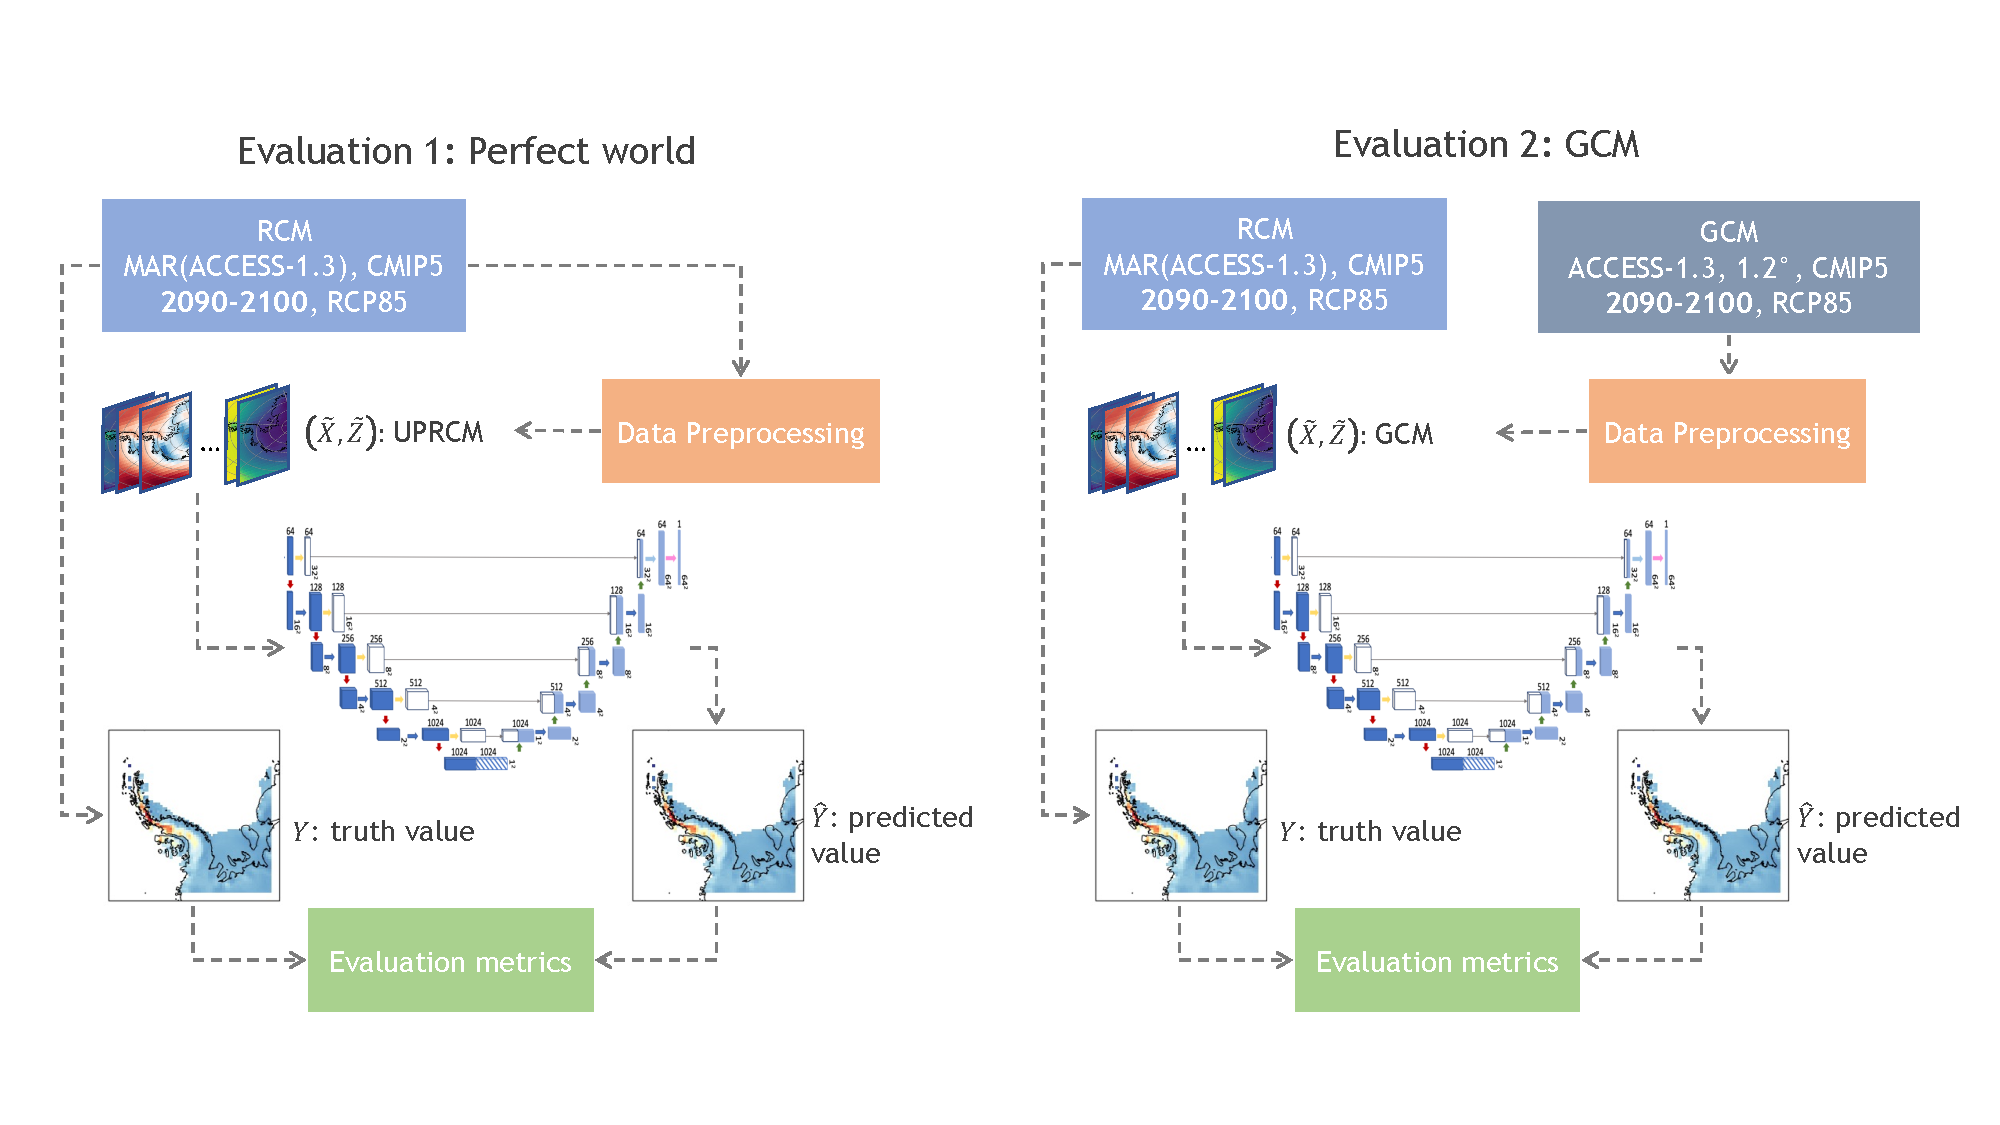
\includegraphics[width=\columnwidth]{doc/Thesis-latex/images/results/evaluation_framework.pdf}
  \caption []{\small Evaluation frameworks. Left: perfect world scenario where the LR input and HR truth given to the Emulator come from the RCM simulation. Right: GCM scenario where LR features come from the GCM and HR truth from the RCM. Evaluation metrics used described in~\ref{subsec:evaluation-metrics}.}
  \vspace{-3mm}
  \label{fig:evaluation-framework}
\end{figure}

\begin{itemize}
    \item Train and test set: we separated the time-frame $T$ into an approximate 90\%-10\% split with a train and test period of $T_{train} = 1980-2090$ and $T_{test} = 2090-2100$. Why? So that the Emulator predicts on features never seen during training.
    We arbitrarily chose to put the test period at the end of the climate model's time-frame out of simplicity, but we could also have taken the test samples elsewhere as long as they are consecutive. 
    \item Evaluation of $\hat{F}_U$: To inspect how the Emulator performs under conditions similar to those of its training, Emulator $\hat{F}_U$ was first evaluated in the perfect model with UPRCM features $\hat{F}_U(\operatorname{UPRCM})$~\cite{Doury}. In a second step, the Emulator is evaluated on GCM inputs $\hat{F}_U(\operatorname{GCM})$. This assesses how the Emulator trained on UPRCM can apply what it learned to GCM features. Furthermore, the performance of $\hat{F}_U(\operatorname{GCM})$ is also a good indicator of the presence of inconsistencies between UPRCM and GCM features. 
    \item Evaluation of $\hat{F}_G$: Because we trained this Emulator on the GCM, we evaluated $\hat{F}_G$ directly on test features from the GCM $\hat{F}_G(\operatorname{GCM})$. 
    \item The two evaluation frameworks are illustrated in Fig.~\ref{fig:evaluation-framework}.
    \item For each Emulator $\hat{F}_{(\cdot)}$, we assessed single month and average predictions made over the target domain. This way, we could examine which regions of the Peninsula were best reconstructed in their SMB patterns in terms of details, precision and intensity. \item Furthermore, we looked at individual time-series of predicted SMB values for single points in the target region. These points were specifically chosen to evaluate how the models handled different patterns and intensities of SMB.   
\end{itemize}

\subsection{Evaluation metrics}\label{subsec:evaluation-metrics} 

To evaluate the global performance of our Machine Learning model, we used different traditional statistics. For each Emulator $\hat{F}_{(\cdot)}$and point $p \in \mathcal{E}$, we compared the target SMB time series $Y_{p}$ to the predicted values $\widehat{Y_{p}}$ over the time period $T_{test}$. We used the Pearson correlation coefficient, RMSE, and Wasserstein distance. Correlation is a good indicator of the reconstruction of temporal patterns such as global global synchrony and seasonality. RMSE and the Wasserstein distance evaluate the fitting of extreme values as a good representation of the monthly variability, and temporal correlation includes a good representation of the extreme values. 

\subsubsection{RMSE}\label{subsubsec:rmse}
Root Mean Squared Error (RMSE) measures the square root of the average squared differences between predicted and target observations. It is also defined as the square of the mean squared error (MSE):
\begin{align}\label{eq:RMSE}
        \operatorname{RMSE}\left(Y_{p},\widehat{Y_{p}}\right) & = \sqrt{\operatorname{MSE}\left(Y_{p},\widehat{Y_{p}}\right)} \\ & = \sqrt{\frac{1}{T}\sum_{t}(\hat{y}_{p}^{t}-y^{t}_{p})^2} & \forall p \in \mathcal{E} 
\end{align}
where $\hat{y}_{p}^{t}$ is predicted SMB value and $y^{t}_{p}$ the true SMB value at location $p\in \mathcal{E} $ and time step $t\in T$. 

\subsubsection{Pearson correlation}\label{subsubsec:pearson-corr}
The Pearson correlation coefficient measures how two continuous time series change over time as a number between -1 (negatively correlated), 0 (uncorrelated), and 1 (perfectly correlated).
\begin{align}
    \operatorname{r}\left(Y_{p},\widehat{Y_{p}}\right) = \frac{\operatorname{cov}(Y_{p},\widehat{Y_{p}})}{\sigma(Y_{p})\sigma(\widehat{Y_{p}})} \;\;\;\; \forall p \in \mathcal{E} 
\end{align}
where $\operatorname {cov}(\cdot)$  is the covariance and  $\sigma(\cdot)$ is the standard deviation.

\subsubsection{Wasserstein distance}\label{subsubsec:wasserstein}
The Wasserstein distance measures the distance between two probability density functions $f(\cdotp)$, in our case $f(Y_p)$ and $f(\widehat{Y_p})$. It is the numerical cost of an optimal transportation problem i.e., the cost of the optimal transport plan~\cite{villani} for moving the mass in the predicted
measure to match that in the target~\cite{wasserstein1}. 
\begin{equation}
    \operatorname{W}\left(f(Y_p),f(\widehat{Y_p})\right) = \sum_{t}|y^{t}_{p}-\hat{y}_{p}^{t}| \;\;\;\; \forall p \in \mathcal{E}
\end{equation}
where $\hat{y}_{p}^{t}$ is the predicted SMB value and $y^{t}_{p}$ the true SMB value at location $p\in \mathcal{E} $ and time step $t\in T$. 

\begin{comment}
 \subsection{Feature importance}\label{subsec:feature-importance}
\begin{itemize}
    \item For each Emulator $\hat{F}_{(\cdot)}$, we were interested in exploring which atmospheric variables had the biggest impact on the performance of the models.
    \item Neural Networks have a reputation of being a black box algorithm with a decision process that is hard to understand. Nevertheless, there are ways to evaluate the importance of features, such as permutation importance. 
    \item Permutation importance is calculated after a model has been fitted. For each single variable in the data, its content are shuffled i.e, rendering the images unreadable and then the model's performance is evaluated with that corrupted variable.
    \item For every variable $x\in C_1$ in the test dataset $X[1:T_{test}, 1:I,1:J,1:C_1]$, we computed the difference between the prediction score on the original data and that of corrupted features. This procedure was repeated $K$ times and the importance was calculated as the mean percentage of difference in scores. 
    \begin{equation}
        \operatorname{I_x} =\frac{1}{K}\sum_{k\in K} \frac{100*(\operatorname{s}_{x}^k - \operatorname{s})}{\operatorname{s}} \;\;\; \forall x\in C_1    \end{equation}
    where $s$ is the NRMSE loss on the original prediction of $\hat{F}_{(\cdot)}$ and $s_x^k$ is the loss for repetition $k\in K$ and corrupted feature $x\in C_1$. 
    \item What is expected: 
    \begin{itemize}
    \item With this technique, we expected to obtain less precise predictions for corrupted features because the resulting data no longer conforms to anything observed by the Emulators~\cite{FeatureImportance2}.
    \item Why? This method breaks the relationship between the features and the target. Because we corrupted the natural structure of the data with our scrambling, we compromised what our model learned during training, resulting in higher errors. Hence the drop in the model score is an indication of how much the model depends on the feature.~\cite{FeatureImportance}
    \end{itemize}
    \item Note that: 
    \begin{itemize}
        \item Permutation importance is not a reflection of the actual predictive value of a feature per se but rather the significance of that feature to a specific model.~\cite{FeatureImportance2}
        \item If two features are correlated and one of them is permuted, the model still has access to this feature via the correlated one. This leads to lower importance for both features, although they might actually be important.~\cite{FeatureImportance2}. 
    \end{itemize}
\end{itemize}
\end{comment}

\chapter{Results}
%%%%%%%%%%%%%%%%%%%%

\begin{itemize}
    \item Flow of Results section:
    \begin{itemize}
    \item Computational efficiency: how much computational power is needed. Why? Whole aim of this model is to be faster and cheaper than the RCM. 
    \item Consistency: Start by evaluating consistency between GCM and UPRCM variables. Why? This way we know how much bias between LR and HR variables the Emulators are dealing with and whether a perfect model framework is necessary. Interesting to know for when UPRCM-Emulator gets GCM inputs and interesting for GCM-Emulator. 
        \item Global ML metrics: move on to evaluate models with metrics over whole target domain. Why? Start global and use typical ML metrics to evaluate performance of models.  
        \item Geoplots: Look at actual prediction images made by Emulators. Why? Good visual aid to assess which regions are best emulated. Can look at details and precision of reconstruction.   
        \item Zoom in on specific points with their time-series and annual SMB values. Why? Look at how the models adapt to different patterns and intensities of SMB. 
    \end{itemize} 
\end{itemize}

\section{Computational efficiency}
\begin{itemize}
\item We trained the Emulators in Pytorch 1.11 on Google Colab's GPU (NVIDIA Tesla K80).
    \item Using early stopping as described in~\ref{subsec:training}, Emulators $\hat{F}_U$ and $\hat{F}_G$ trained for $31$ and $40$ epochs before stopping. Training took approximately $4$ minutes with roughly $6$ seconds per epoch. A GPU is no longer needed once the Emulator is trained, and prediction on test data takes $15$ seconds on a CPU, which is nearly instantaneous. 
    \item This computational time is significantly smaller than running an RCM simulation as that can take several weeks to calculate on a super-computer~\cite{Doury}. 
    \item Note that our computational time does not include the preparation of data for the Emulator, but if the data is readily obtainable and a correct data processing pipeline is in place, selecting the target region and creating the UPRCM takes only a few hours on a CPU.   
\end{itemize}



\section{Bias between RCM and GCM variables}\label{sec:res-bias-RCM-GCM}
To assess the bias and inconsistencies between the large-scale and fine-scale atmospheric variables, we calculated the temporal and spatial correlation between UPRCM and GCM features (Eq.~\ref{eq:spatial-corr} and Eq.\ref{eq:temporal-corr}). Results can be seen in Fig.~\ref{fig:corr-GCM-RCM}. 
\begin{itemize}
    \item Fig.~\ref{fig:temp-corr-GCM-UPRCM}: 
    \begin{itemize}
        \item For most of the atmospheric variables, the time-series of URPCM and GCM features are highly positively correlated, with values very close to $1$. 
        \item However, the two wind variables (EW, NW) show inconsistencies between large and local scale time-series over the mainland and Peninsula with minimal correlation values reaching $0.2$.
        \item This suggests that, except for winds, there is almost no inconsistency in the seasonal patterns between regional and global variables. 
    \end{itemize}
    \item Fig.~\ref{fig:spatial-corr-GCM-UPRCM} and Fig.~\ref{fig:spatial-corr-GCM-RCM-ex}: 
    \begin{itemize}
        \item As seen in Fig.~\ref{fig:spatial-corr-GCM-UPRCM}, variables like temperature, specific humidity, radiation, and precipitation show significant changes in spatial correlation between UPRCM and GCM features.
        \item The most flagrant variables are SWD, with an annual pattern strongly oscillating between approximate spatial correlation values of $0.2$ and $0.8$, and precipitation with a very poor correlation.
        \item Looking at some individual examples in Fig.~\ref{fig:spatial-corr-GCM-RCM-ex}, we see that the spatial correlation is low for SWD radiation during winter because the GCM predicts higher radiation values in the mainland than RCM. However, because there is very little radiation, spatial correlation is high in summer. 
        \item For precipitation, the patterns in the UPRCM and GCM are very different, with the RCM being much more precise in its predictions. For example, for November, the UPRCM shows a local high-intensity precipitation region on the tip of the Peninsula, while the GCM predicts a more imprecise pattern of lower intensity. 
        \item We also notice a streak pattern on the left boundary of the RCM, but this is a known problem as the boundaries of climate models are usually imprecise. 
    \end{itemize}
    \item Overall, we found problems in consistency between large and local-scale variables. As mentioned in~\ref{subsec:perfect-model}, these biases might confuse an Emulator, and this might justify the usage of the perfect model framework for training a model. 
\end{itemize}


\begin{figure}[tbp]
        \centering
        \begin{subfigure}[b]{\columnwidth}
            \centering 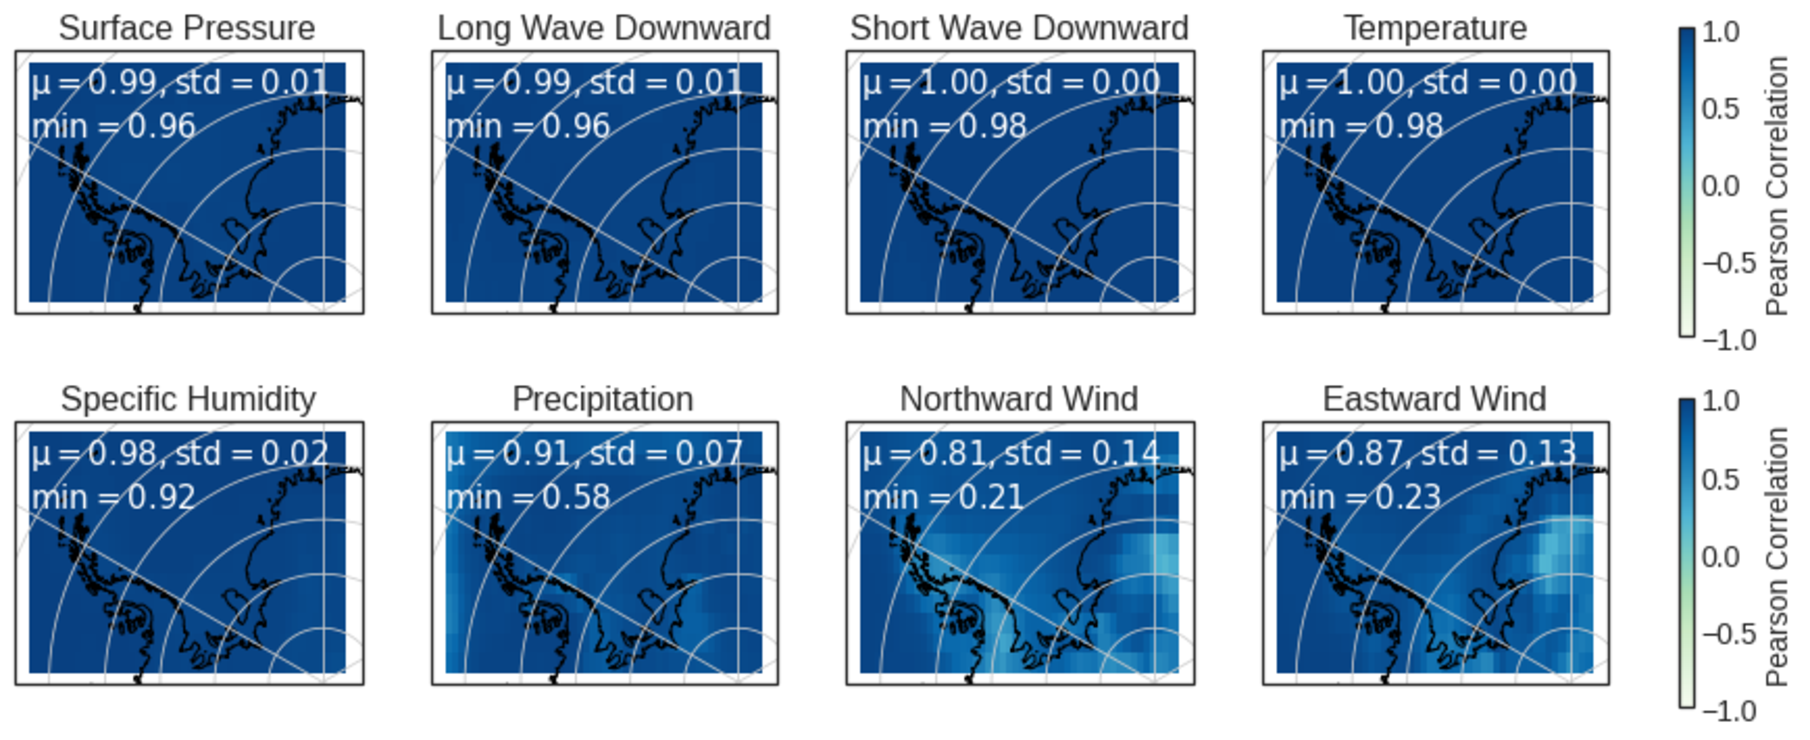
\includegraphics[width=\textwidth]{doc/Thesis-latex/images/results/temporalCorr_RCM_GCM.pdf}
            \caption[]%
            {{\small Temporal correlation over test period}}    
          \label{fig:temp-corr-GCM-UPRCM}
        \end{subfigure}
        \hfill
            \begin{subfigure}[b]{\columnwidth}
            \centering 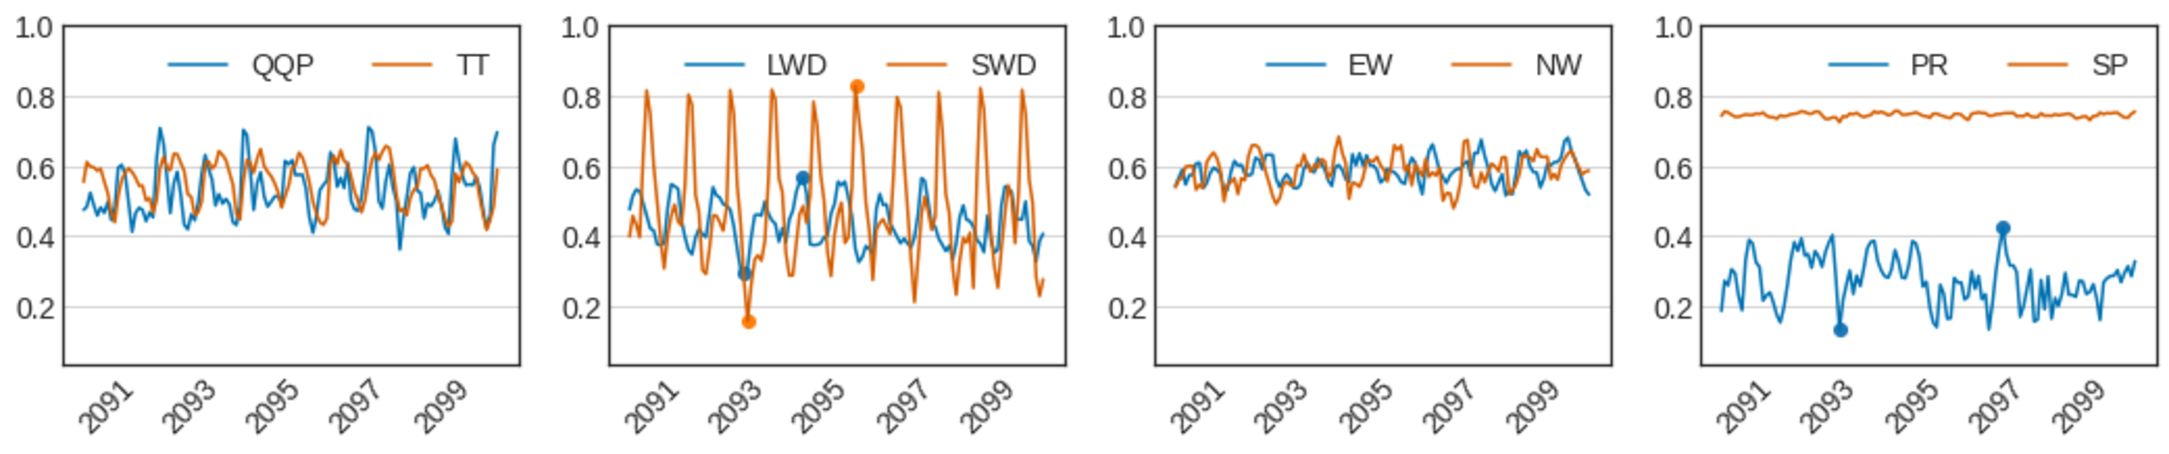
\includegraphics[width=\textwidth]{doc/Thesis-latex/images/results/spatialCorr_TS_RCM_GCM.pdf}
            \caption[]%
            {{\small Spatial correlation over test period}}    
          \label{fig:spatial-corr-GCM-UPRCM}
        \end{subfigure}
        \hfill
        \begin{subfigure}[b]{\columnwidth}  
            \centering 
            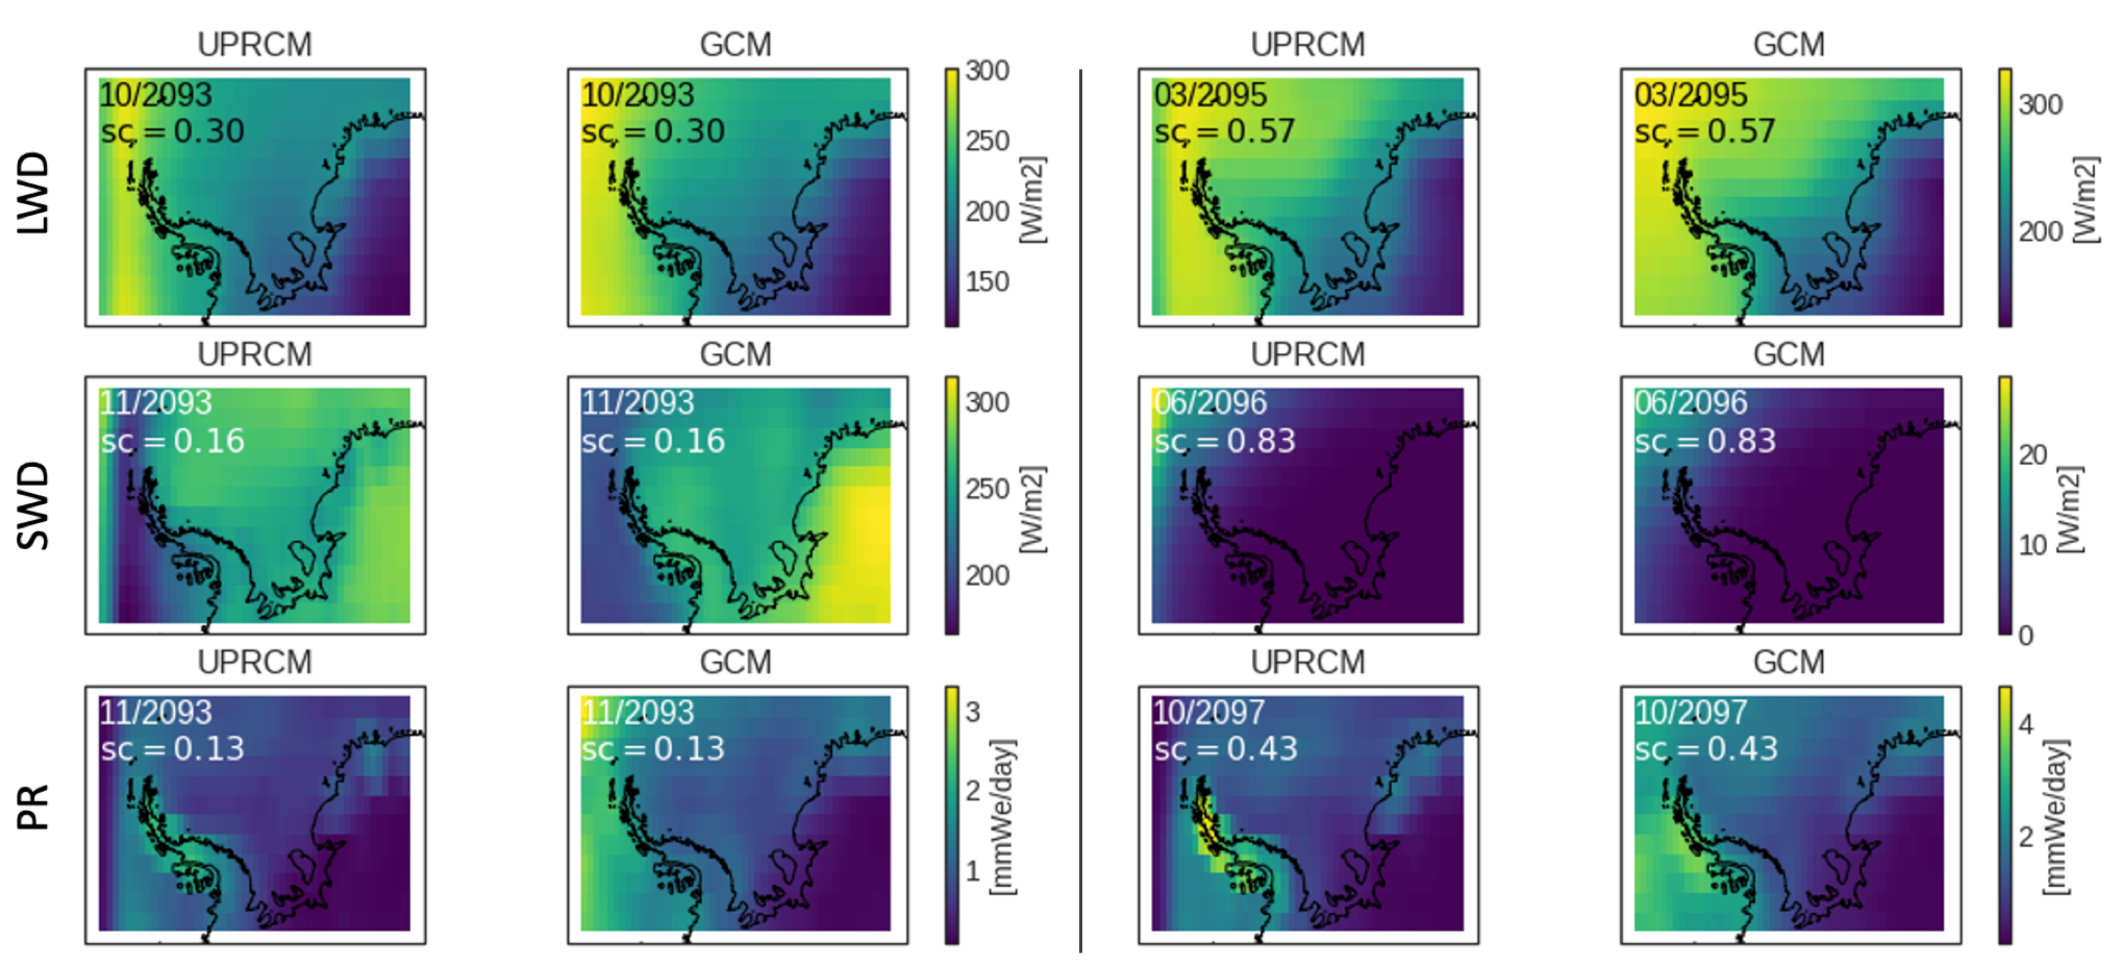
\includegraphics[width=\textwidth]{doc/Thesis-latex/images/results/spatialCorr_RCM_GCM.pdf}
            \caption[]%
            {{\small Spatial correlation for individual variables and months}} \label{fig:spatial-corr-GCM-RCM-ex}
        \end{subfigure}
        \hfill
        \caption[]
        {\small Temporal (a) and spatial (b, c) correlation between UPRCM and GCM variables given as input to Emulator ($\hat{F}$) over target domain ($\mathcal{E})$) and test period (2090-2100). (a) Temporal correlation between UPRCM and GCM time-series for each point $p$ in target domain $\mathcal{E}$. Legend: mean ($\mu$) and standard deviation ($\operatorname{std}$) over $\mathcal{E}$. (b) Spatial correlation between UPRCM and GCM variables over $\mathcal{E}$ for each time step. (c) Example of time steps with lowest (left) and highest (right) spatial correlation ($\operatorname{sc}$) between UPRCM and GCM. Variables from top to bottom: long-wave downward radiation (LWD), short-wave downward radiation (SWD) and precipitation (PR).} 
        \label{fig:corr-GCM-RCM}
    \end{figure}

%%%%%%%%%%%%%%%%%%%%


\section{Evaluation metrics}
To evaluate the overall performance of both Emulators, we used three traditional machine learning metrics as described in~\ref{subsec:evaluation-metrics}. Results can be seen in Fig.~\ref{fig:evaluation-GCM-RCM}. Here we were particularly interested in seeing how the metrics differ for regions with high amplitudes of SMB i.e., regions with high precipitation, such as the tip and west-coast, and dryer regions such as the east-coast and mainland. 
\begin{itemize}
    \item Pearson correlation coefficient: As seen in the box-plot, in average, $\hat{F}_{U}(UPRCM)$ and $\hat{F}_{G}(GCM)$ show higher correlation values than $\hat{F}_{G}(GCM)$. This is especially illustrated on the tip and west coast of the peninsula, where $\hat{F}_{U}(UPRCM)$ and $\hat{F}_{G}(GCM)$ show the highest correlation to the truth, with values close to 1. The east coast of the peninsula has the lowest correlations, especially for $\hat{F}_{G}(GCM)$. We suspect this is because the model struggles to emulate temporal SMB patterns of dry regions such as the inland and east peninsula. 
    \item Wasserstein distance and RMSE: With the highest Wasserstein distance and RMSE values, $\hat{F}_{U}(GCM)$ shows that the density probability functions of the emulated SMB series are farther from the RCM truth when given GCM inputs than UPRCM. For this particular Emulator, the peninsula shows high differences in distributions with outliers with significant scores up to $10$ for Wasserstein distance and $14$ for RMSE. This hints that the Emulator $\hat{F}_{U}(GCM)$  struggles to reach high SMB intensities when given GCM inputs while trained on UPRCM.   
    \item Overall, we see that according to these metrics, $\hat{F}_{U}(UPRCM)$ and $\hat{F}_{G}(GCM)$ perform very similarly and always perform better than $\hat{F}_{U}(GCM)$. While temporal patterns and seasonality are best reconstructed in regions of high precipitation such as the tip and west-coast of the peninsula, the Emulators struggle to emulate their extreme values, especially $\hat{F}_{U}(GCM)$. 
\end{itemize}


% evaluation metrics
\begin{figure}[!ht]
  \centering
  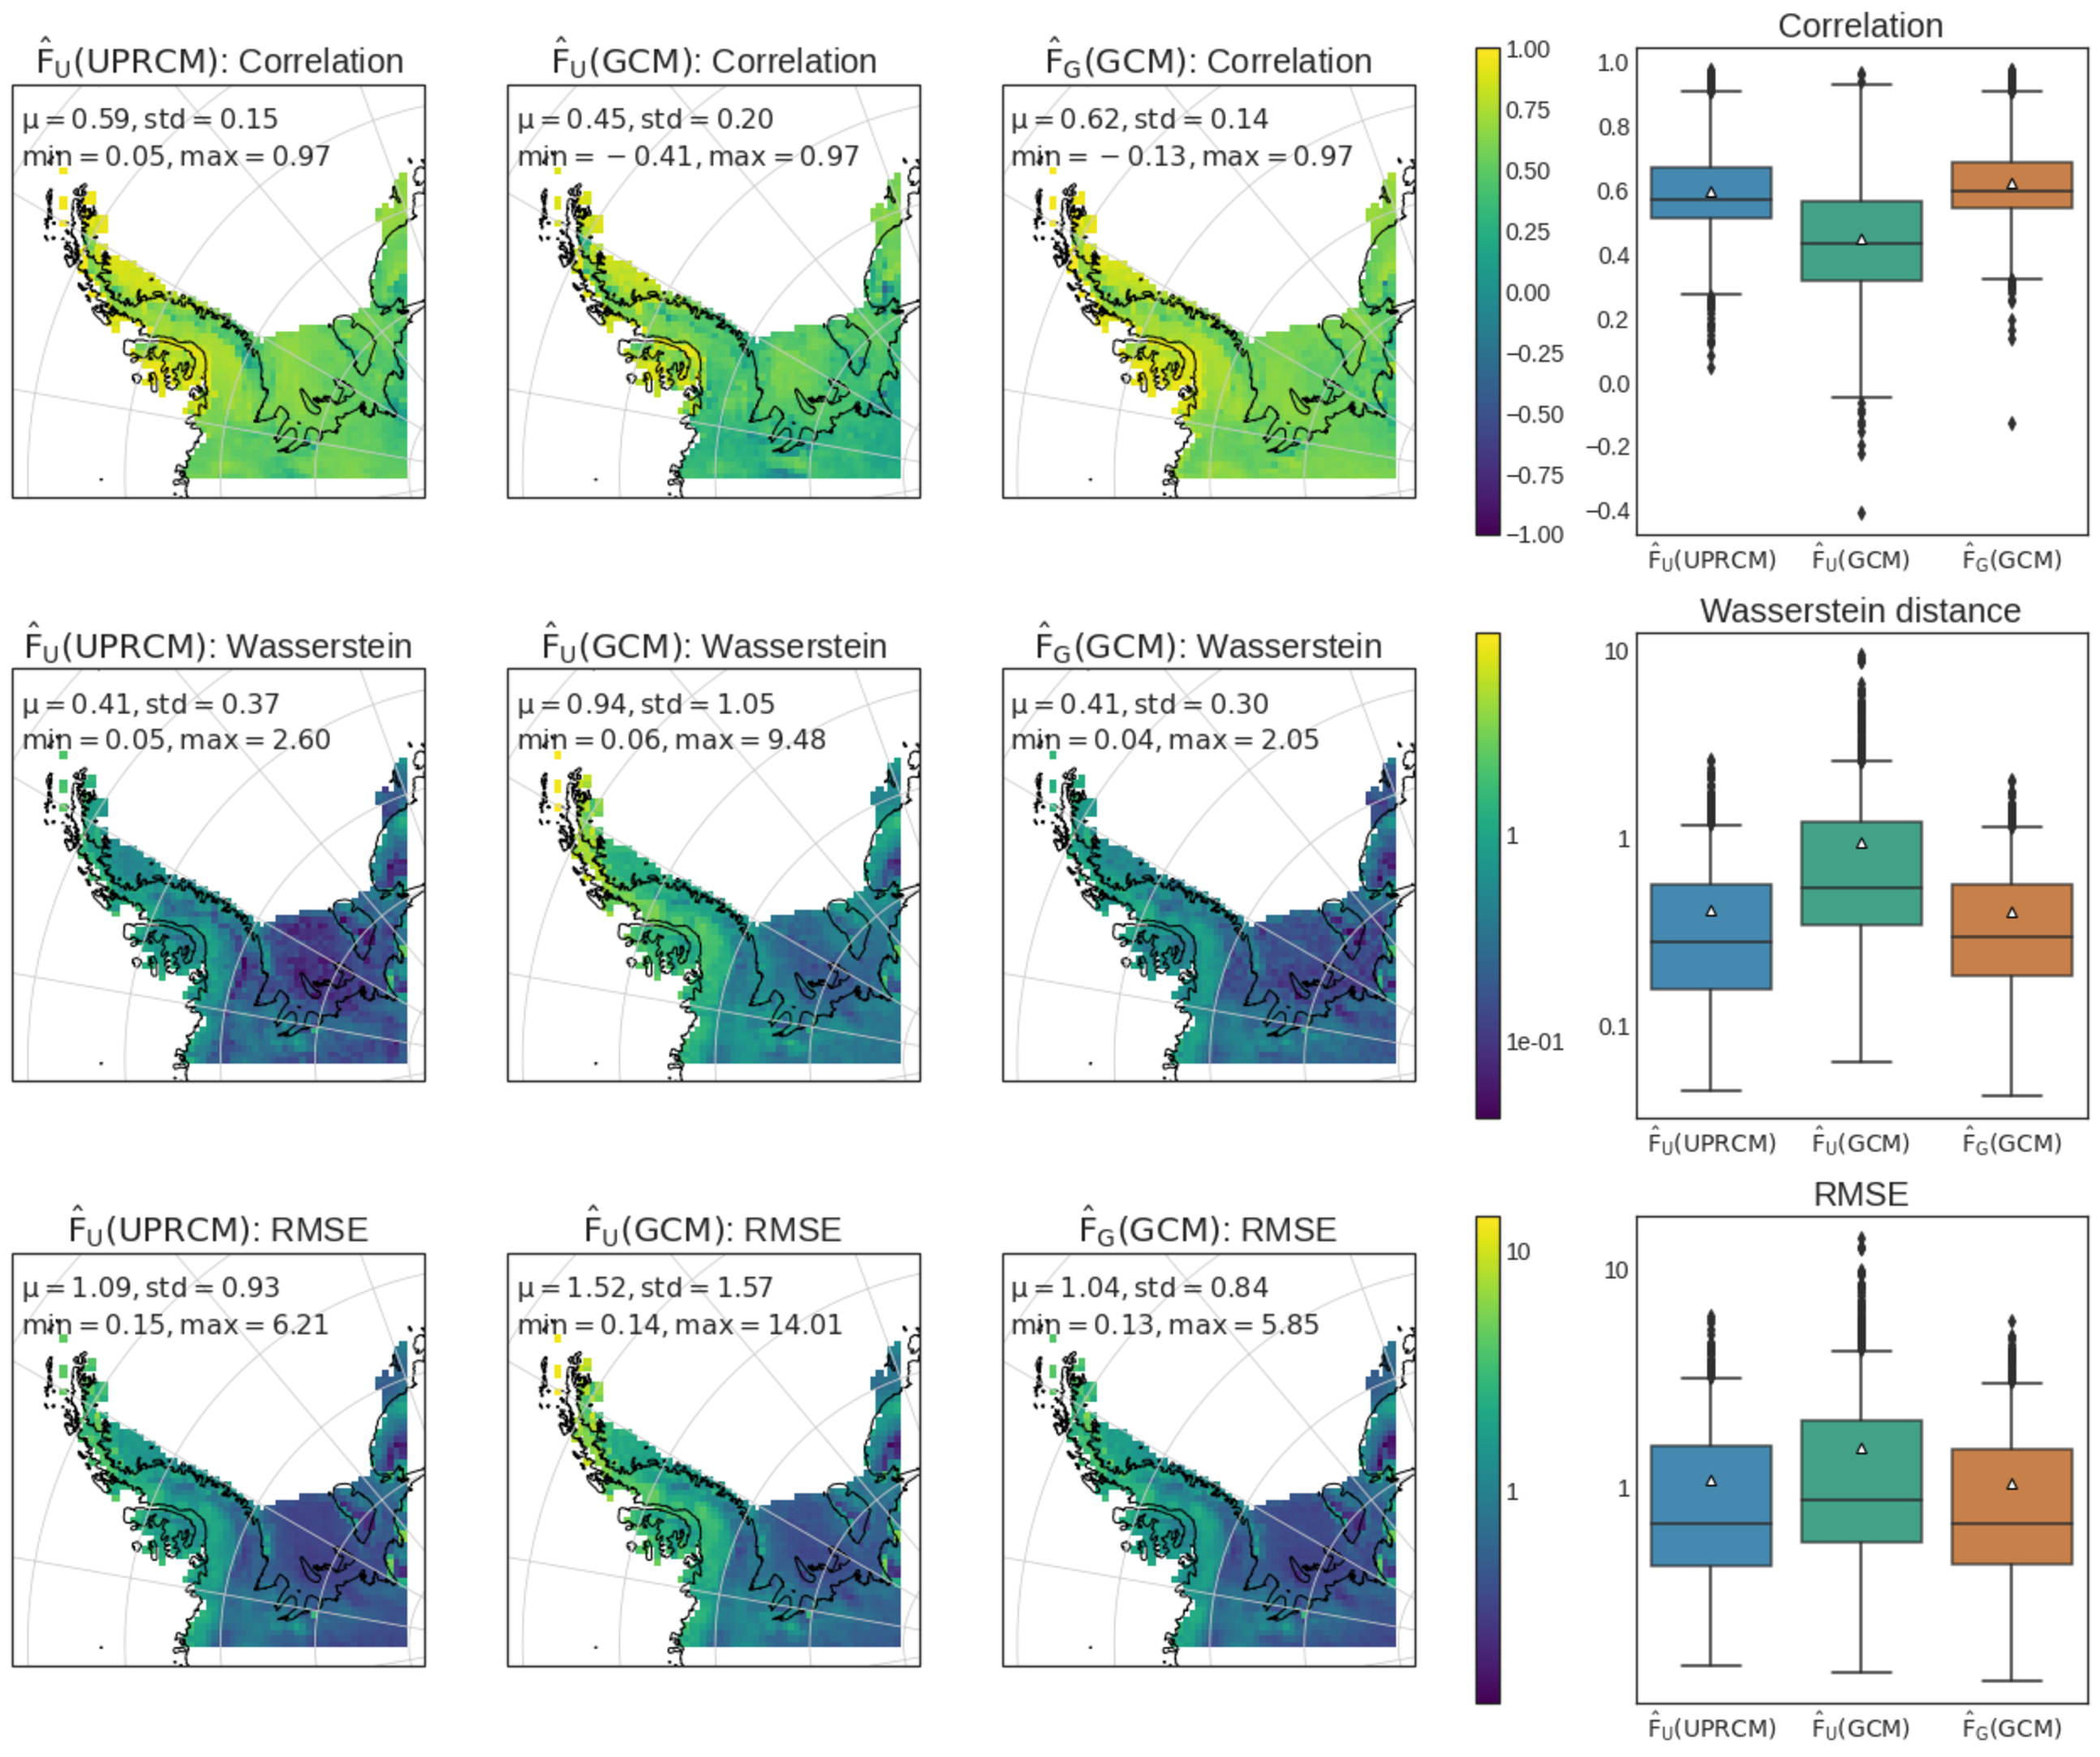
\includegraphics[width=\columnwidth]{doc/Thesis-latex/images/results/metrics_RCM_GCM.pdf}
  \caption []{\small Evaluation of Emulator trained on UPRCM ($\hat{F}$) or on GCM ($\hat{G}$) and using respectively UPRCM ($\operatorname{\hat{F}(UPRCM)}$) and GCM as low-resolution input ($\operatorname{\hat{F}(GCM)}$, $\operatorname{\hat{G}(GCM)}$). Test period (2090-2100). At each position $p$ in target domain $\mathcal{E}$, the truth series over the test period are compared to predicted SMB values $\operatorname{\hat{F}(\cdot)}$ and $\operatorname{\hat{G}(\cdot)}$. Right: box plot of evaluation metric values, extending from lower to upper quartile, with a line at the median and triangle at the mean. From top to bottom: Pearson correlation, Wasserstein distance and RMSE (\ref{subsubsec:rmse}). Legend: spatial mean ($\operatorname{\mu}$) and standard deviation ($\operatorname{std}$) of metric over $\mathcal{E}$. }
  \vspace{-3mm}
  \label{fig:evaluation-GCM-RCM}
\end{figure}


\subsection{Geoplots}
To evaluate how our models emulate spatial structures, we compare a prediction for a random month and average predictions over the test period to the target RCM. Results can be seen in Fig.~\ref{fig:geoplots-GCM-RCM}. 
\begin{itemize}
    \item Unsurprisingly, in the first two columns in Fig.~\ref{fig:geoplots-GCM-RCM} we see that compared to the low-resolution UPRCM map, the high-resolution RCM truth is more detailed and has a more complex spatial structure. As expected, because of their precipitation patterns, we see that the tip and west coast of the peninsula show strong values in SMB, some points reaching $10$ \si{[mmWe/day]}. 
    \item For the chosen random month, except for higher intensity regions in the mainland, $\hat{F}_{U}(UPRCM)$ and $\hat{F}_{G}(GCM)$ competently reproduce the spatial structure of the RCM truth. Both have a very small RMSE, which becomes even smaller when looking at the average prediction over the test period ($0.09$ and $0.08$). On average, both models' predictions look similar to the average target RCM. 
    \item However, $\hat{F}_{U}(GCM)$, both for the random month and on average, is not able to reproduce the extreme values of SMB and creates a toned-down version of the truth. This is reflected in its RMSE, which is twice as high as the other two models ($0.53$ for a random month and $0.23$ on average). 
    \item Overall, this Figure hints that both Emulators, when evaluated on data similar to what they were trained on, have a solid capacity to reproduce the complex spatial structures of RCM. 
\end{itemize}

% SMB predictions over geoplots
\begin{figure}[thb]
  \centering
  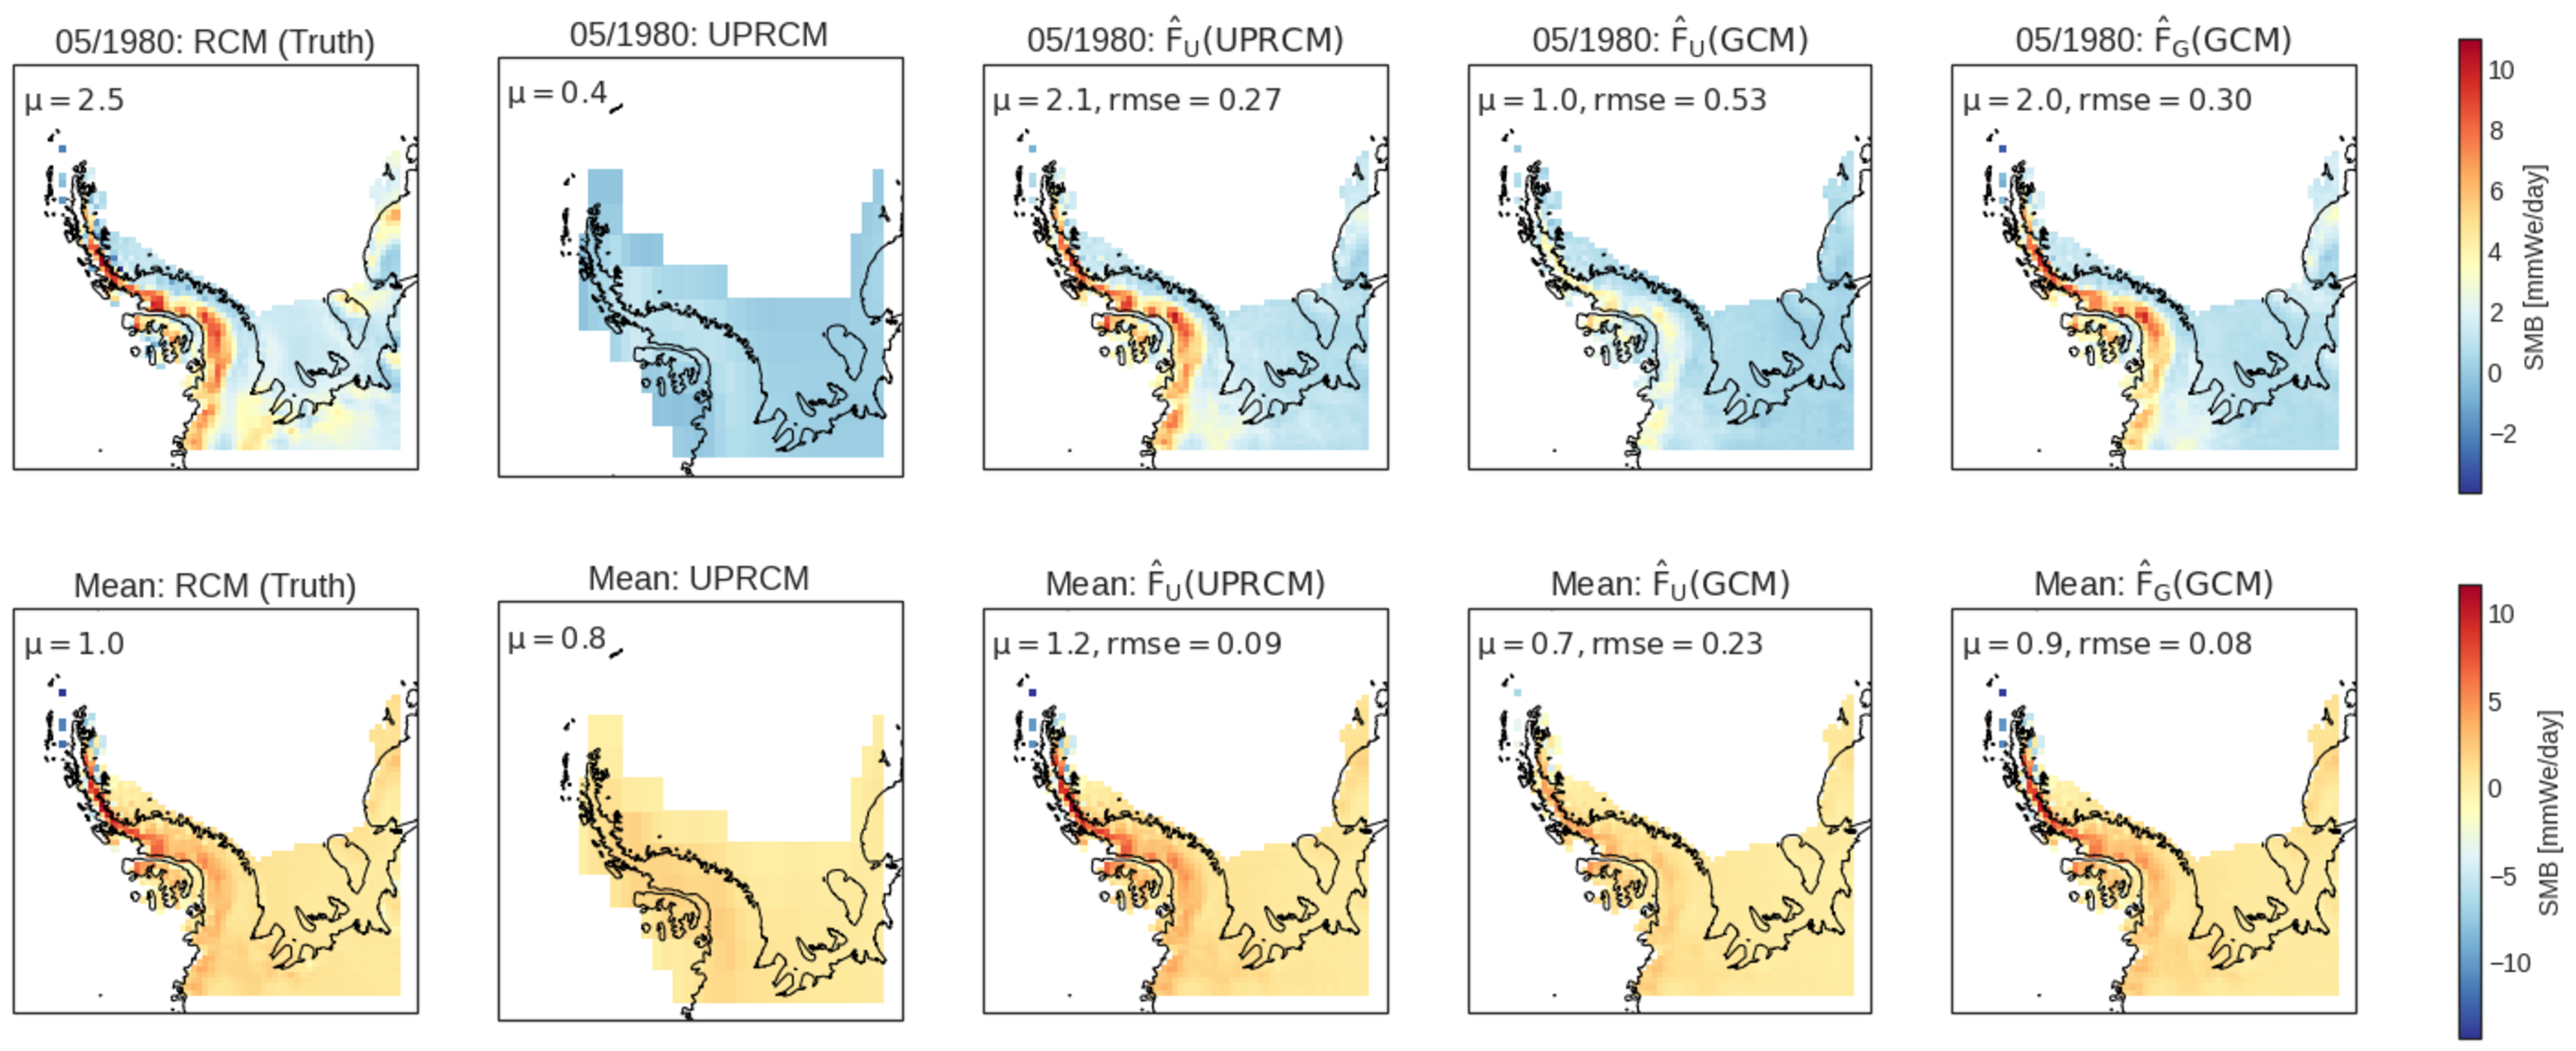
\includegraphics[width=\columnwidth]{doc/Thesis-latex/images/results/geoplots_RCM_GCM.pdf}
  \caption []{\small SMB on a random month (05/1980) (top) and averaged over the test period (bottom) over $\mathcal{E}$. From left to right: SMB as in the UPRCM, true RCM, $\operatorname{\hat{F}(UPRCM)}$ and $\operatorname{\hat{F}(GCM)}$. Legend: spatial mean ($\mu$) over $\mathcal{E}$ and spatial RMSE ($\operatorname{rmse}$) between the emulated and true SMB pixel values.}
  \vspace{-3mm}
  \label{fig:geoplots-GCM-RCM}
\end{figure}

\subsection{Time-series}\label{sec:res-time-series}
To assess how the Emulators predict different patterns and intensities of SMB, we plotted the emulated time series for four geographical points (Fig.~\ref{fig:points-location}). First, we chose two points in regions with higher levels of precipitation: P1 on the Larsen C ice-shelf whose SMB values annually oscillate between $-5$ and $5$ \si{[mmWe/day]} and P2 on the west coast, that once per year reaches low extremes of $-15$ \si{[mmWe/day]}. On the other side, P4 on the Ronne ice-shelf has a significantly drier climate ($0-1.5$ \si{[mmWe/day]}). Finally, we chose P3 on the east coast for its drier weather ($0-4$ \si{[mmWe/day]}) and its temporal SMB pattern that looks less seasonal than the other three points. Time series and annual predictions for each point can be seen in Fig.~\ref{fig:timeseries-GCM-UPRCM}. 
\begin{itemize}
    \item For each of these 4 points, $\hat{F}_{U}(UPRCM)$ and $\hat{F}_{G}(GCM)$ come very close to reproducing the patterns of the RCM truth series. 
    \item For P1 and P2, all emulators capture the seasonality pattern well, with high correlation values (close to $1$ for P2). $\hat{F}_{G}(GCM)$ looks like it is even a little bit better than $\hat{F}_{U}(UPRCM)$ at emulating low drops and high peaks in SMB. 
    \item For P3 and P4, even if they miss a few of the peaks, $\hat{F}_{U}(UPRCM)$ and $\hat{F}_{G}(GCM)$ show a good ability for reproducing the time-series pattern, even when their behavior is less cyclical, like for P3. However, for P4, we notice that the Emulators struggle when faced with multiple close peaks per year and merge them into one prominent peak. 
    \item As was already seen in Fig.~\ref{fig:geoplots-GCM-RCM}, $\hat{F}_{U}(GCM)$ struggles to reproduce high amplitude values, and this is very noticeable in its time series. They capture the seasonal patterns (reflected in a high correlation) but produce a toned-down version of the RCM truth time series (reflected in a higher RMSE).
    \item This behavior is also reflected in the annual SMB predictions for all models. $\hat{F}_{U}(UPRCM)$ and $\hat{F}_{G}(GCM)$ come very close to the true annual SMB values, with $\hat{F}_{G}(GCM)$ again a little bit better than $\hat{F}_{U}(UPRCM)$ for almost all years. However, $\hat{F}_{U}(GCM)$ on average consistently underestimates the truth by half. 

\end{itemize}


% Time series and geoplots for four points
\begin{figure}[tbp]
        \centering
        \begin{subfigure}[b]{0.2\columnwidth}
            \centering 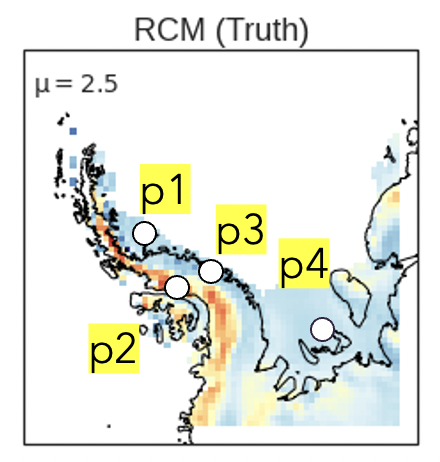
\includegraphics[width=\textwidth]{doc/Thesis-latex/images/results/points_location.png}
            \caption[]%
            {{\small}}    
          \label{fig:points-location}
        \end{subfigure}
        \hfill
        \begin{subfigure}[b]{\columnwidth}  
            \centering 
           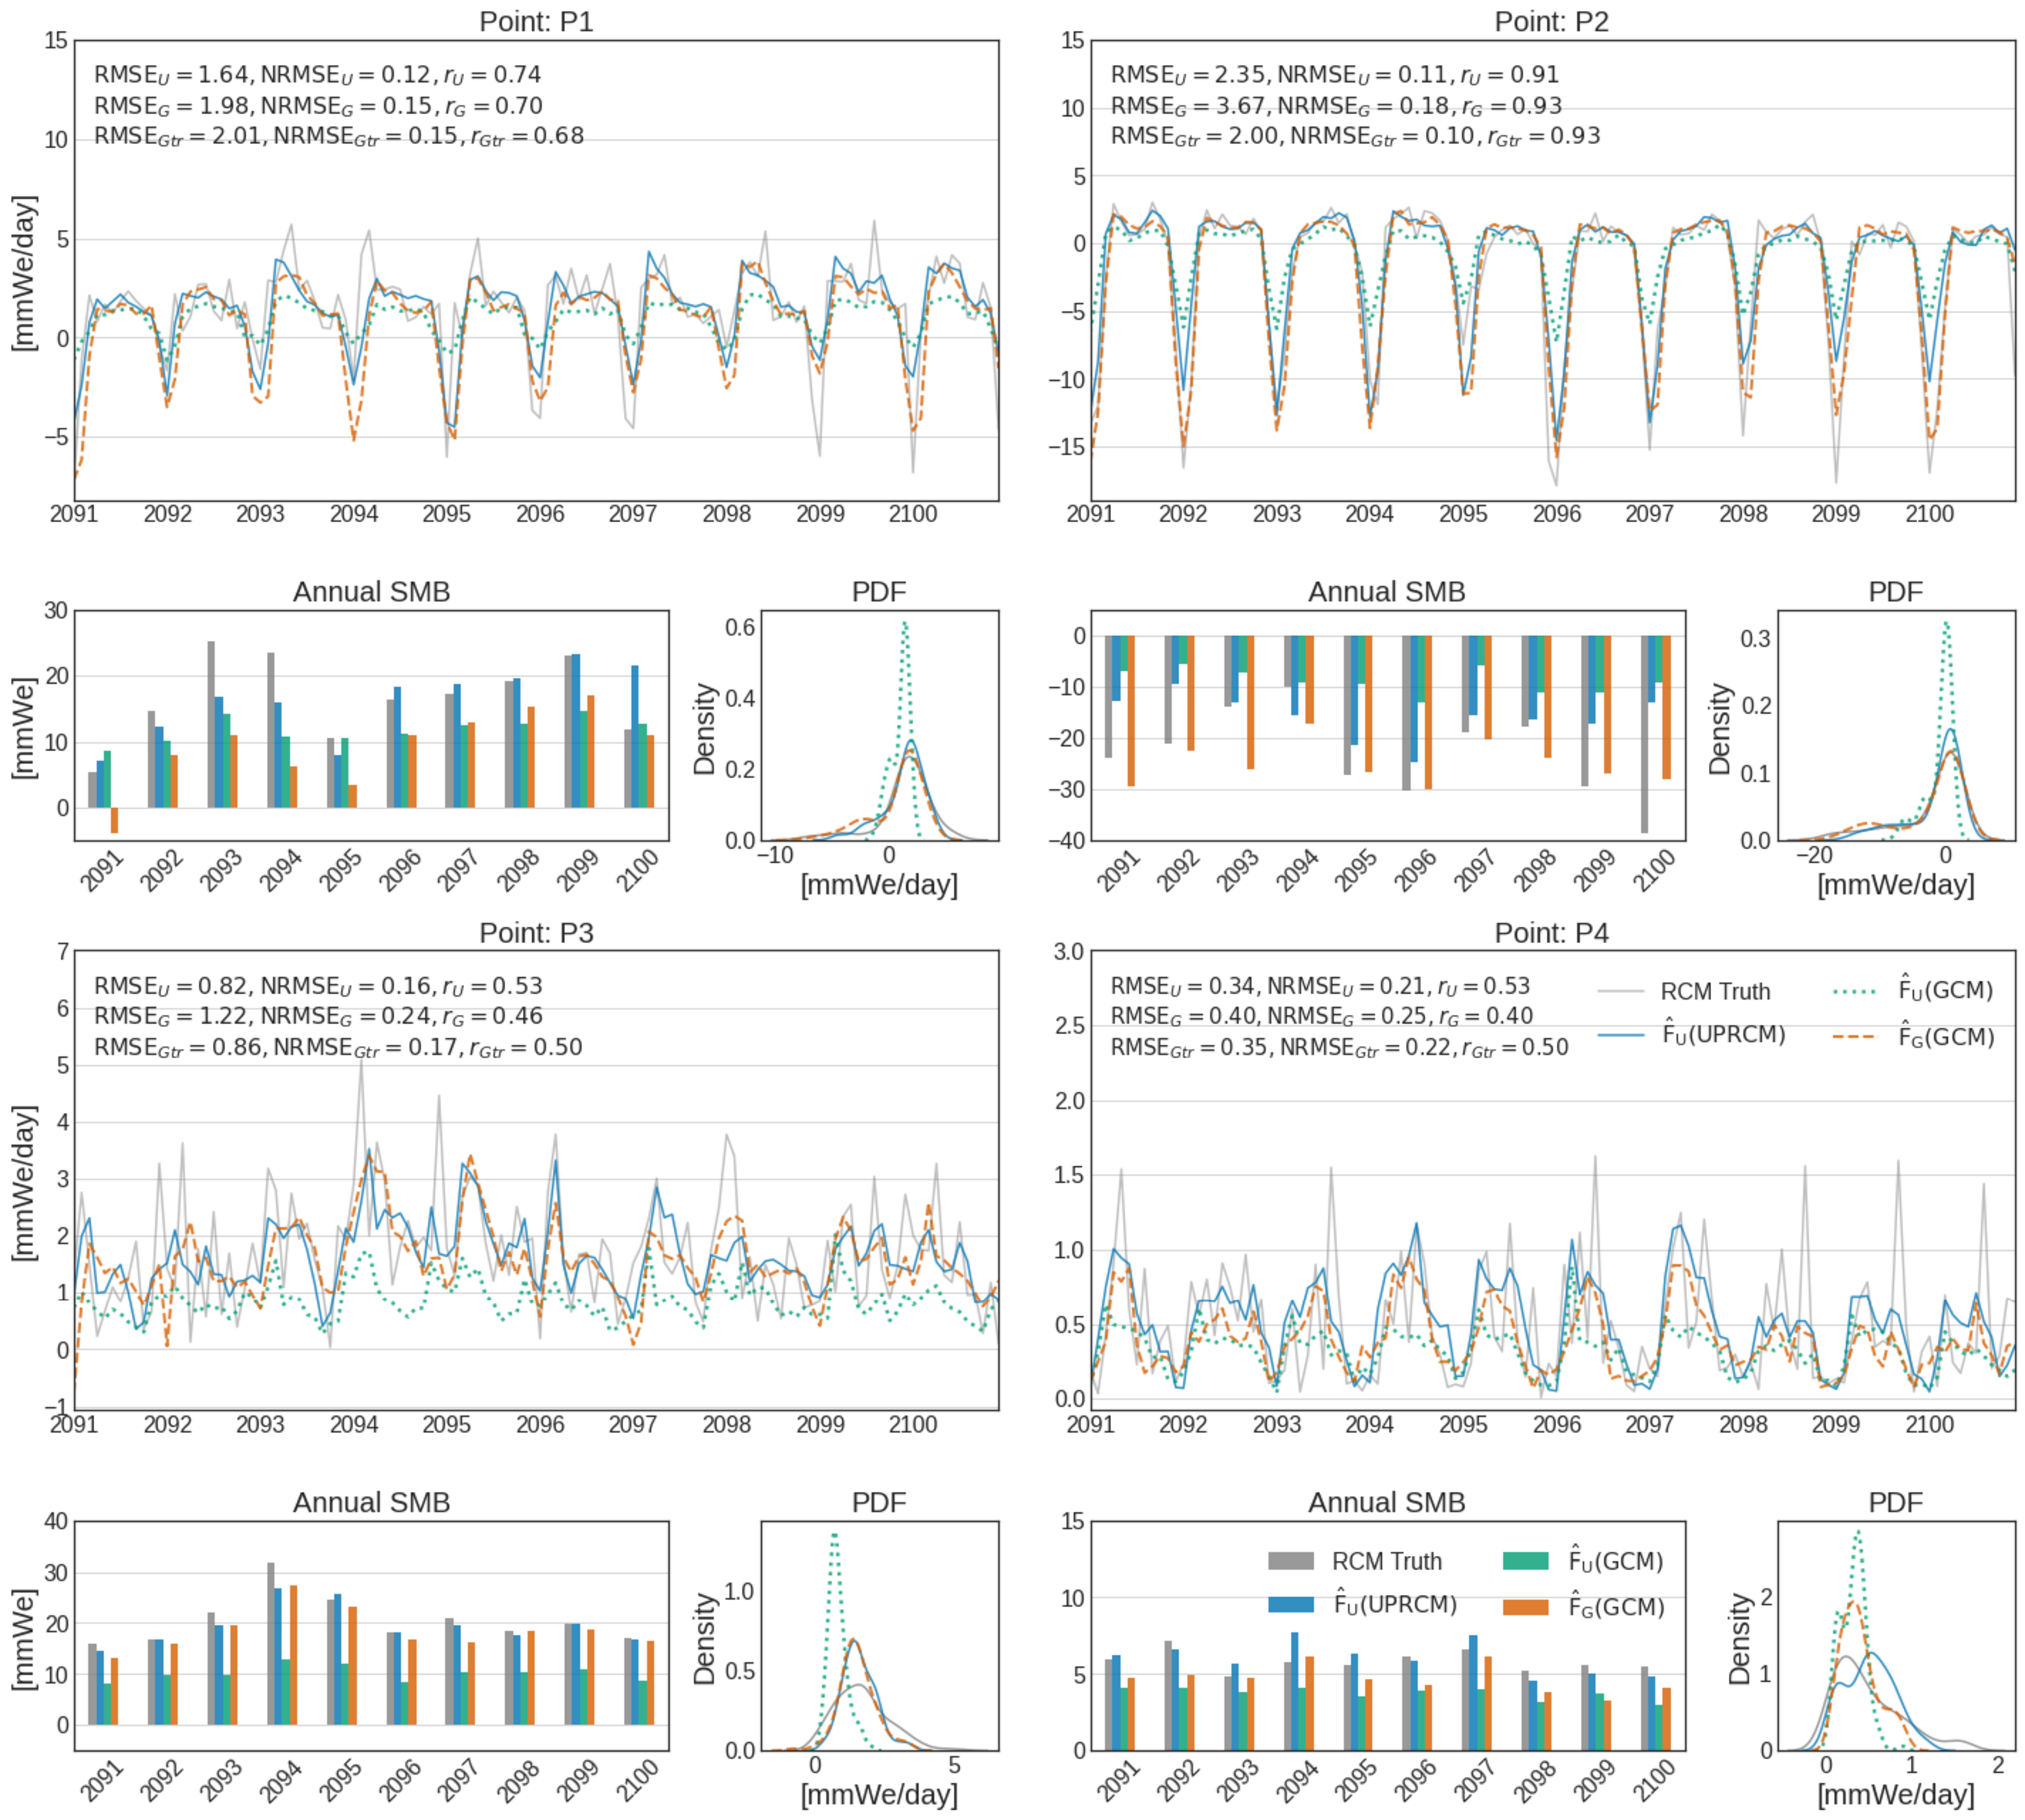
\includegraphics[width=\textwidth]{doc/Thesis-latex/images/results/timeseries_RCM_GCM.pdf}
            \caption[]%
            {{\small }}  
          \label{fig:timeseries-GCM-UPRCM}
        \end{subfigure}
        \hfill
        \caption[]
        {\small SMB predictions of Emulators $\operatorname{\hat{F}_{U}(UPRCM)}$ (blue line), $\operatorname{\hat{F}_{U}(GCM)}$ (dotted green) and $\operatorname{\hat{F}_{G}(GCM)}$ (dashed orange) compared to RCM Truth (grey line). (b) Time-series of predictions of Emulator for four different geographical points (a) in target domain $\mathcal{E})$. Legend: temporal correlation ($\operatorname{r}$), temporal RMSE ($\operatorname{RMSE}$) and NRMSE ($\operatorname{NRMSE}$) between the time-series of emulated and true SMB. $U$ = $\operatorname{\hat{F}_{U}(UPRCM)}$, $G$ = $\operatorname{\hat{F}_{U}(GCM)}$ and $Gtr$ = $\operatorname{\hat{F}_{G}(GCM)}$. Test time-frame: 2090-2100. } 
        \label{fig:points-timeseries-GCM-UPRCM}
    \end{figure}

\begin{comment}

\subsection{Feature importance}
To have an indicator of which atmospheric variables have the biggest impact on the Emulators' performance, we explored feature importance according to the algorithm outlined in~\ref{subsec:feature-importance}. 
\begin{itemize}
    \item Correlation between variables: first, we calculated correlation between atmospheric variables themselves. As outlined in ~\ref{subsec:feature-importance}, having two variables with a high correlation between them might lead to lower importance for individual variables.  
\end{itemize}

% Feature importance
\begin{figure}[tbp]
        \centering
        \begin{subfigure}[b]{\columnwidth}
            \centering 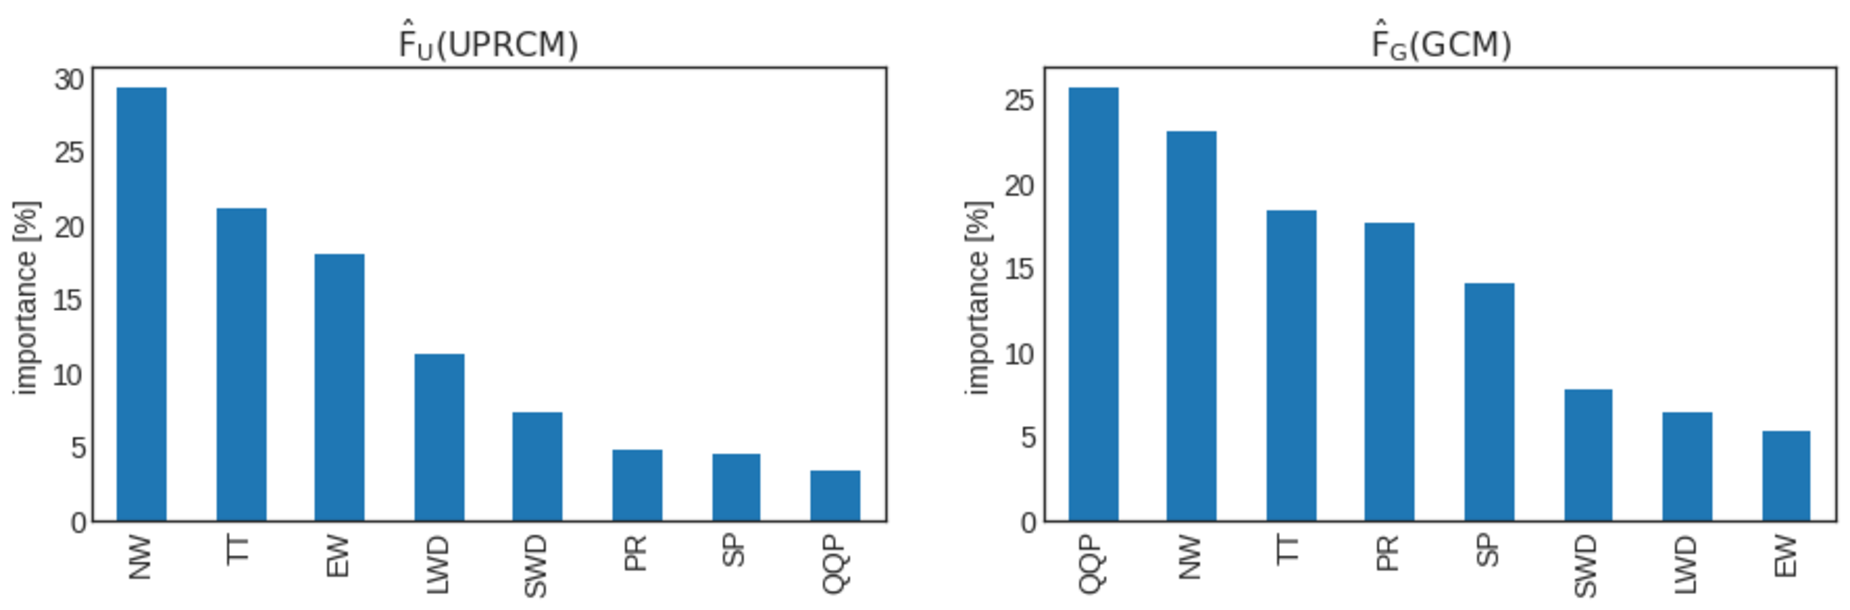
\includegraphics[width=\textwidth]{doc/Thesis-latex/images/results/feature_importance.pdf}
            \caption[]%
            {{\small Feature importance for $\hat{F}_U(UPRCM)$, $\hat{F}_U(GCM)$ and  $\hat{F}_G(GCM)$}}    
          \label{fig:points-location}
        \end{subfigure}
        \hfill
        \begin{subfigure}[b]{0.8\columnwidth}  
            \centering 
           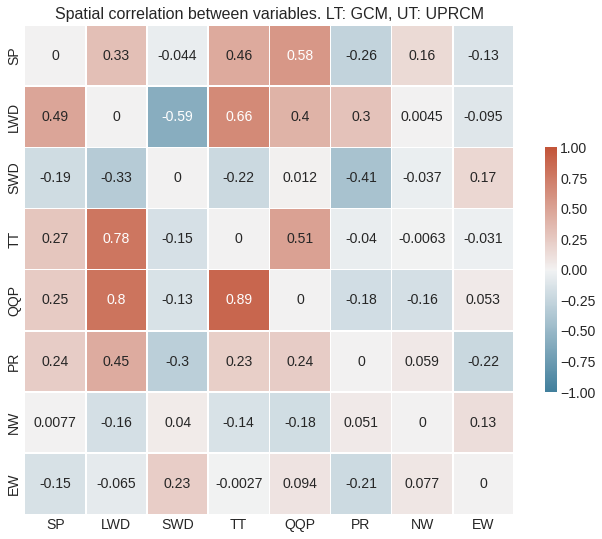
\includegraphics[width=\textwidth]{doc/Thesis-latex/images/results/correlation_between_variables.png}
            \caption[]%
            {{\small }}  
          \label{fig:timeseries-GCM-UPRCM}
        \end{subfigure}
        \hfill
        \caption[]
        {\small Predictions of Emulator trained on UPRCM ($\hat{F}$) or on GCM ($\hat{G}$) and using respectively UPRCM ($\operatorname{\hat{F}(UPRCM)}$) and GCM as low-resolution input ($\operatorname{\hat{F}(GCM)}$, $\operatorname{\hat{G}(GCM)}$). (b) Time-series of predictions of Emulator for four different geographical points (a) in target domain ($\mathcal{E})$). True SMB (grey), $\operatorname{\hat{F}(UPRCM)}$ (blue), $\operatorname{\hat{F}(GCM)}$ (green) and $\operatorname{\hat{G}(GCM)}$ (orange). Legend: temporal correlation ($\operatorname{r}$) and temporal RMSE ($\operatorname{RMSE}$) between the time-series of emulated and true SMB. Test time-frame: 2090-2100. } 
        \label{fig:points-timeseries-GCM-UPRCM}
    \end{figure}
\end{comment}

\chapter{Discussion}
%%%%%%%%%%%%%%%%%%%%
Discussion section flow:
\begin{itemize}
    \item Extension of Emulator on temperature to SMB. Why? What is different from emulating near-surface temperature, what are its limitations. Does it work to change it from temperature to SMB? 
    \item Perfect model framework. Why? Discuss utility of perfect model framework and its extension when trained on GCM. Is tit really useful or can we just train directly on the GCM?  
    \item Utility of Emulator. Why? Is it really faster and easier to use than computing an RCM? 
\end{itemize}

\section{Extending the Emulator of near-surface temperature over France to SMB over Antarctica}\label{sec:extension-doury}
\begin{itemize}
    \item In this study, we extended the machine learning model that emulated near-surface temperature over the south of France, proposed in~\cite{Doury}. 
    \item In doing this, we were faced with several challenges as SMB is notoriously challenging to observe and represent in models compared to temperature~\cite{Lenaerts}. 
    \begin{itemize}
        \item HR variable not in LR input: Because temperature is a variable in the GCM and RCM, it was present in the low-resolution features given as input to the model in~\cite{Doury}. In our case, SMB was only available in the RCM. Thus, our Emulator could exclusively reconstruct a high-resolution SMB image given a limited number of other atmospheric variables. This might explain why some regions in the Antarctic Peninsula, especially those with less seasonal patterns, might be harder for the model to reconstruct. We rely on the assumption that our model has a clear physical relationship to learn between our eight large-scale atmospheric variables and local scale SMB, but this might not be true for all points. 
        \item Space variations: Ice sheet SMB varies highly across multiple space and time scales, while temperature tends to be a more stable and seasonal variable. For example, as was discussed in~\ref{sec:res-time-series}, on the Antarctic Peninsula, while some regions have high seasonal amplitude changes in SMB, others have almost none. If they do, it is only with very little difference in amplitude. This was not the case for the near-surface temperature emulated in~\cite{Doury}, where, even though their target domain covered different climates, its temperature fluctuated in approximately the same annual amplitude range for all points in their domain. Compared to their model, ours, therefore, had to acclimate different scales in SMB values over the Peninsula. For this, we used a normalized RMSE loss, but our model still better emulates regions with high seasonal change, hinting that NRMSE might not be enough to account for different scales in target values. 
    \end{itemize}
    \item Even if our Emulator can still be improved, especially when considering regions with dry climates, for the rest it can reproduce the temporal variability and spatial structure of SMB nearly perfectly for both $\hat{F}_{U}(UPRCM)$ and $\hat{F}_{G}(GCM)$. Therefore, by extending the model proposed in~\cite{Doury}, with slight modifications, it is possible to emulate SMB over the Antarctic Peninsula. 
\end{itemize}

\section{On the usage of the perfect model framework}\label{sec:disc-perfect-model}
As outlined in~\ref{subsec:training}, we trained two Emulators separately, one following the perfect model framework proposed in~\cite{Doury} and another directly on GCM data. 
\begin{itemize}
    \item Emulator trained on UPRCM but evaluated on GCM: 
    \begin{itemize}
        \item The authors of ~\cite{Doury} state that the perfect model framework is necessary to learn the RCM downscaling function without any interfering biases between GCM and RCM. However, to be useful, the Emulator should give correct predictions of SMB when given large-scale GCM variables as input. Nevertheless, while $\hat{F}_{U}(GCM)$ predictions follow the correct temporal patterns, they consistently underestimate the true SMB values and produces a toned-down version of the RCM truth time-series.
        \item Under the perfect model framework, the Emulator cannot learn large-scale GCM-RCM inconsistencies during its training. Consequently, when the model is given GCM inputs, GCM-RCM inconsistencies are preserved and appear in the predictions~\cite{Doury}.
    \end{itemize}
    \item Existence of bias: As shown in~\ref{sec:res-bias-RCM-GCM}, we find significant bias and inconsistencies between RCM and GCM variables. For example, the two wind variables showed high temporal discrepancies between large and local-scale simulations. This might happen if there is an offset in the RCM time-series compared to the GCM or if the patterns are completely different. Furthermore, we also found spatial patterns inconsistencies for most atmospheric variables, especially for precipitation and radiation. Some of this bias might exist for problematic reasons, such as inconsistent forcings or boundary conditions when RCM simulations are computed~\cite{Doury, Laprise2008ChallengingST}. For example, we suspect these might be the reasons for the streaks visible on the left boundary of RCM images. However, we assume that the rest of the RCM-GCM inconsistencies exist because the RCM revises the low-resolution simulation for valid reasons, i.e., for a more refined representation of the physical processes~\cite{Doury}. 
     \item Emulator trained on GCM: For this reason, we trained a second Emulator directly on GCM inputs to see whether it could account for the GCM-RCM bias. While $\hat{F}_{G}(GCM)$ misses some precision in emulating SMB patterns compared to $\hat{F}_{U}(UPRCM)$ for regions with minor SMB variations, it comes very close to the RCM truth for the rest. It is also performing exceedingly well in terms of predicting annual SMB values and is significantly better than $\hat{F}_{U}(GCM)$. 
     \item Under the assumption that most of the GCM-RCM exists for valid reasons, it seems like the perfect model framework may not be necessary to train an Emulator. The model, when trained on GCM data, can predict SMB values close to the truth, as if it learned the underlying RCM-GCM inconsistencies and dynamics.   
\end{itemize}


\section{Usage of the Emulator}\label{sec:utility-emulators}
For the Emulator to be practical, it has to be faster and easier to use than computing an RCM simulation. We showed in the results section that if the pre-processing data pipeline is not too time-consuming, then training the Emulator and making predictions is very fast, with predictions made nearly instantaneously. However, we still need to explore how easy the model is to use.  
\begin{itemize}
    \item Transparency: Neural networks have a reputation for being a black box algorithm with a decision process that is hard to understand. This is not different in our case. Because we give all available variables to our model without making any uphill feature selection, it would be interesting to know which physical features carry the most weight in the model's decision. Though now there are new ways to try to "open the black box"~\cite{Guidotti, Doury}, it remains a challenging problem for which we, unfortunately, did not have more time to explore. So while traditionally computing an RCM allows the user to have complete control over the variables, forcings, boundary conditions, etc., using a machine learning Emulator offers less transparency.  
    \item Randomness and reproducibility: training a neural network while relying on a GPU creates several sources of randomness. To make our model reproducible, we used a fixed seed, and in this setting, our model always gives the same predictions. Nevertheless, another seed might provide very different results, so to reproduce our results, one must be careful to use the same random settings. To assess the robustness of our Emulator, one could run it several times using different seeds and observe the average results. Due to time constraints, this was omitted. 
    \item Specificity of model: 
    \begin{itemize}
        \item Other regions: our model focuses only on one target region, the Antarctic Peninsula. If one wanted to expand it to other areas, one would have to re-train the model on data of this specific region. We suspect that applying our Emulator elsewhere would not work otherwise, as it would be faced with images very different from its training. However, we believe that because the Emulator works well for the Peninsula, an area that shows high variability in SMB patterns, it will perform just as well for other domains of Antarctica once it has been correctly trained. 
        \item Other simulations: just as for another target domain, if one wanted to extend the Emulator to other climate model simulations, one would need to re-train it for those climate models. One exception might be if they are very similar to ACCESS 1.3 and MAR(ACCESS 1.3). For example, one could try making predictions with the Emulator on another future RCP simulation of the MAR(ACCESS 1.3) e.g., RCP 4.5 instead of RCP 8.5.  
    \end{itemize}
    \item Availability of data: the ACCESS 1.3 GCM data is openly available to the public on the Australian NCI
    website~\cite{NCI}. However, we had to ask for the MAR(ACCESS 1.3) RCM data from the Geo-science Institute of the University of Grenobles. Therefore, while acquiring GCM data is easy, getting access to RCM simulations might be more difficult.   
\end{itemize}
Overall, while the Emulator is very fast in training and prediction, the primary time bottle-neck is getting the correct data and pre-processing it to fit the desired training setting.  


%%%%%%%%%%%%%%%%%%%%
\chapter{Conclusion}
%%%%%%%%%%%%%%%%%%%%
\begin{itemize}
    \item The idea of Emulator: In this study, we built a machine learning model called the Emulator that emulates local-scale surface mass balance (SMB) values over the Antarctic Peninsula by learning the downscaling function of a regional climate model (RCM). This means that our model, when given low-resolution atmospheric variables from a global climate model (GCM), can reconstruct a high-resolution image of SMB from a regional climate model. Compared to an RCM, the Emulator is designed to be computationally cheaper and faster.   
    \item How the Emulator was built: Our model is an extension of a U-Net model proposed in~\cite{Doury} that emulated near-surface temperature over the south of France. We extended their U-net by adding attention mechanisms in the Encoder of the U-Net and replaced traditional convolutional operations with depthwise-separable convolutions. Furthermore, to account for the different scales of SMB values across the Antarctic Peninsula, we change the original MSE loss to a normalised RMSE. 
    \item Training setting: For training our model, we propose two frameworks. The first follows the perfect model framework from~\cite{Doury} where the Emulator receives low-resolution inputs from the RCM instead of the GCM. For this, we create large-scale features from RCM with interpolation. This setting is designed so that the model learns the downscaling function undisturbed by potential RCM-GCM inconsistencies and biases. In the second framework, we train the model on large-scale features directly sourced from the GCM to evaluate whether it can learn those inconsistencies. 
    \item Computational speed: Training our model takes under ten minutes on a GPU, and predictions are almost instantaneous, but data gathering and pre-processing can be time-consuming. However, our Emulator is significantly faster than an RCM simulation, which can take several weeks on a supercomputer. 
    \item Evaluation of the Emulators:
    \begin{itemize}
        \item We evaluate the first Emulator, trained in the perfect model setting, on large-scale features from the RCM, and in a second step, directly with variables from the GCM. While the Emulator evaluated on RCM features can almost perfectly reproduce the high-resolution SMB truth, predictions made with GCM features consistently underestimate it. This is not surprising as we find significant spatial and temporal bias while exploring the consistency between GCM and RCM features. Because the the perfect model framework does not allow the Emulator to learn large-scale GCM-RCM inconsistencies, they are conserved when predicting with GCM variables, leading to underestimation. 
        \item The second Emulator, trained directly on GCM features, can reproduce detailed high-resolution SMB maps. The model can make correct annual SMB predictions and reconstruct the temporal patterns of individual SMB time-series and global spatial structures over the Antarctic Peninsula. Its only limitation is producing an accurate representation of points in dry climates where NRMSE loss is insufficient to account for the small SMB values. In further work, one could focus on these climates to improve the Emulator's predictions. 
        
        Assuming that RCM-GCM inconsistencies exist for a valid reason and that we wish the Emulator to account for them, our results indicate that a perfect model framework might not be needed and that our model can learn them.  
    \end{itemize}
    
In conclusion, we build an machine learning RCM-Emulator that can predict SMB over the Antarctic Peninsula significantly faster than computing an RCM simulation. 
\end{itemize}

\section{Code availability}
All notebooks and python scrips for pre-processing and machine learning are available on our \href{https://github.com/marvande/master-thesis}{GitHub} repository~\cite{GitHub}. For any questions or additional information about the code, email: \href{mailto:marijn.vandermeer@bluewin.ch}{marijn.vandermeer@bluewin.ch}. 

\cleardoublepage
\phantomsection
\addcontentsline{toc}{chapter}{Bibliography}
\printbibliography
% %%%%%%%%%%%%%%%%%%%%%%%%%%%%%%%%%%%%%%
% Appendices are optional
\appendix

\chapter{Data processing}
All pre-processing of the GCM is done on Pangeo, a community platform for Big Data geoscience. 
\section{Pre-processing of the GCM}\label{sec:preproc-GCM}
\begin{itemize}
    \item We downloaded the ACCESS 1.3 data from~\cite{NCI}. We chose the dataset with atmospheric variables (Amon) for CMIP5 and r1i1p1 ensemble. We downloaded the historical and future simulation RCP 8.5, which are monthly mean aggregations of daily values. The data can also be directly downloaded with the wget script on our \href{https://github.com/marvande/master-thesis}{GitHub}. 
    \item From this dataset, we chose the eight variables as seen in Table~\ref{tab:features}. 
    \item Antarctica: To restrict the dataset size and because we were only interested in Antarctica, we cut the GCM data so that its latitude was between $-40$ and $-90$ $\degree C$. 
    \item Reprojecting: because the GCM is in latitude-longitude coordinates, but the RCM is in polar stereographic coordinates, we reprojected the GCM to the same projection system as the RCM. We did this by upsampling the RCM stereographic grid to cover approximately the same resolution as the GCM, and we interpolated the GCM on that grid. 
    \item Units: for the following variables, the units were changed so that they coincided with the RCM. 
    \begin{itemize}
        \item Precipitation: from \si{kg m^{-2}s^{-1}} to \si{mmWe/day}
        \item Pressure: from \si{pa} to \si{hpa}
        \item Temperature: from \si{K} to \si{C}
        \item Specific humidity: from \si{g/g} to \si{g/Kg}
    \end{itemize}
    \item Smoothing average: GCM outputs were smoothed by a 3x3 moving average filter to follow the same procedure as in~\cite{Doury}. 
\end{itemize}

\section{Pre-processing of the RCM}\label{sec:preproc-RCM}
\begin{itemize}
    \item Because the GCM data we had was in monthly frequency, we did a monthly mean aggregation for the RCM data. We also changed the spatial units from \si{km} to \si{m} to be in accordance with GCM units. 
    \item Surface values: variables like the winds, temperature, and specific humidity were provided for seven pressure levels while we needed surface-level values. Pressure levels were: 200, 500, 600, 700, 800, 850, 925 \si{hpa}. Each pressure level had NaN values where it intersected with the surface. Therefore, for each point $p$ in the RCM domain, we took the last non-NaN value on the highest possible pressure level as the surface value.  
    \item Winds: RCM winds variables were given as x and y-components while GCM winds were Northward and Eastward. Therefore RCM wind components needed to be reprojected to become North/Eastward winds. First we calculated a grid that gave the latitude ($\mathrm{lat}$) and longitude ($\mathrm{lon}$) coordinates for each point $(i,j)\subset X,Y $ in the RCM polar stereographic grid. Then, for each point $(i,j)$ we applied Algorithm~\ref{alg:wind-components}.  
    
    \begin{algorithm}
    \caption{Transformation of wind components into Northward-Eastward winds}\label{alg:wind-components}
    \begin{algorithmic}[1]
    \State $\operatorname{GEddxx} = 90$
    \State $\Delta \phi = 90 - \operatorname{GEddxx}$
    \State $dr = \pi / 180$ 
    \For{$i,j \in X,Y$}
    \State $\phi \gets -1*dr*(\mathrm{lon}[i,j] + \Delta \phi)$
    \State $\mathrm{cphi} \gets cos(-\phi)$
    \State $\mathrm{sphi} \gets sin(-\phi)$
    \State  $\mathrm{windEast}[i, j] \gets \mathrm{cphi} * \mathrm{windX}[i, j] - \mathrm{sphi} * \mathrm{windY}[i,j]$ \Comment{Eastward wind component}
    \State $\mathrm{windNorth}[i, j] \gets  \mathrm{sphi} * \mathrm{windX}[i, j] + \mathrm{cphi} * \mathrm{windY}[i, j]$ \Comment{Northward wind component}
    \EndFor
    \end{algorithmic}[1]
    \end{algorithm}
    
    \item Creation of UPRCM: to create GCM-like low-resolution features from the RCM, we reprojected the RCM on the GCM grid by interpolation. Then, we used the same moving average filter for the GCM to smooth the data (Fig.~\ref{fig:training-data-flow}). Finally, because there is no precipitation variable in the RCM, we created one by adding the snowfall and rainfall variables. 
    \begin{equation}
        \mathrm{PR} = \mathrm{SF} + \mathrm{RF}
    \end{equation}
\end{itemize}

\begin{figure}[!htb]
  \centering
  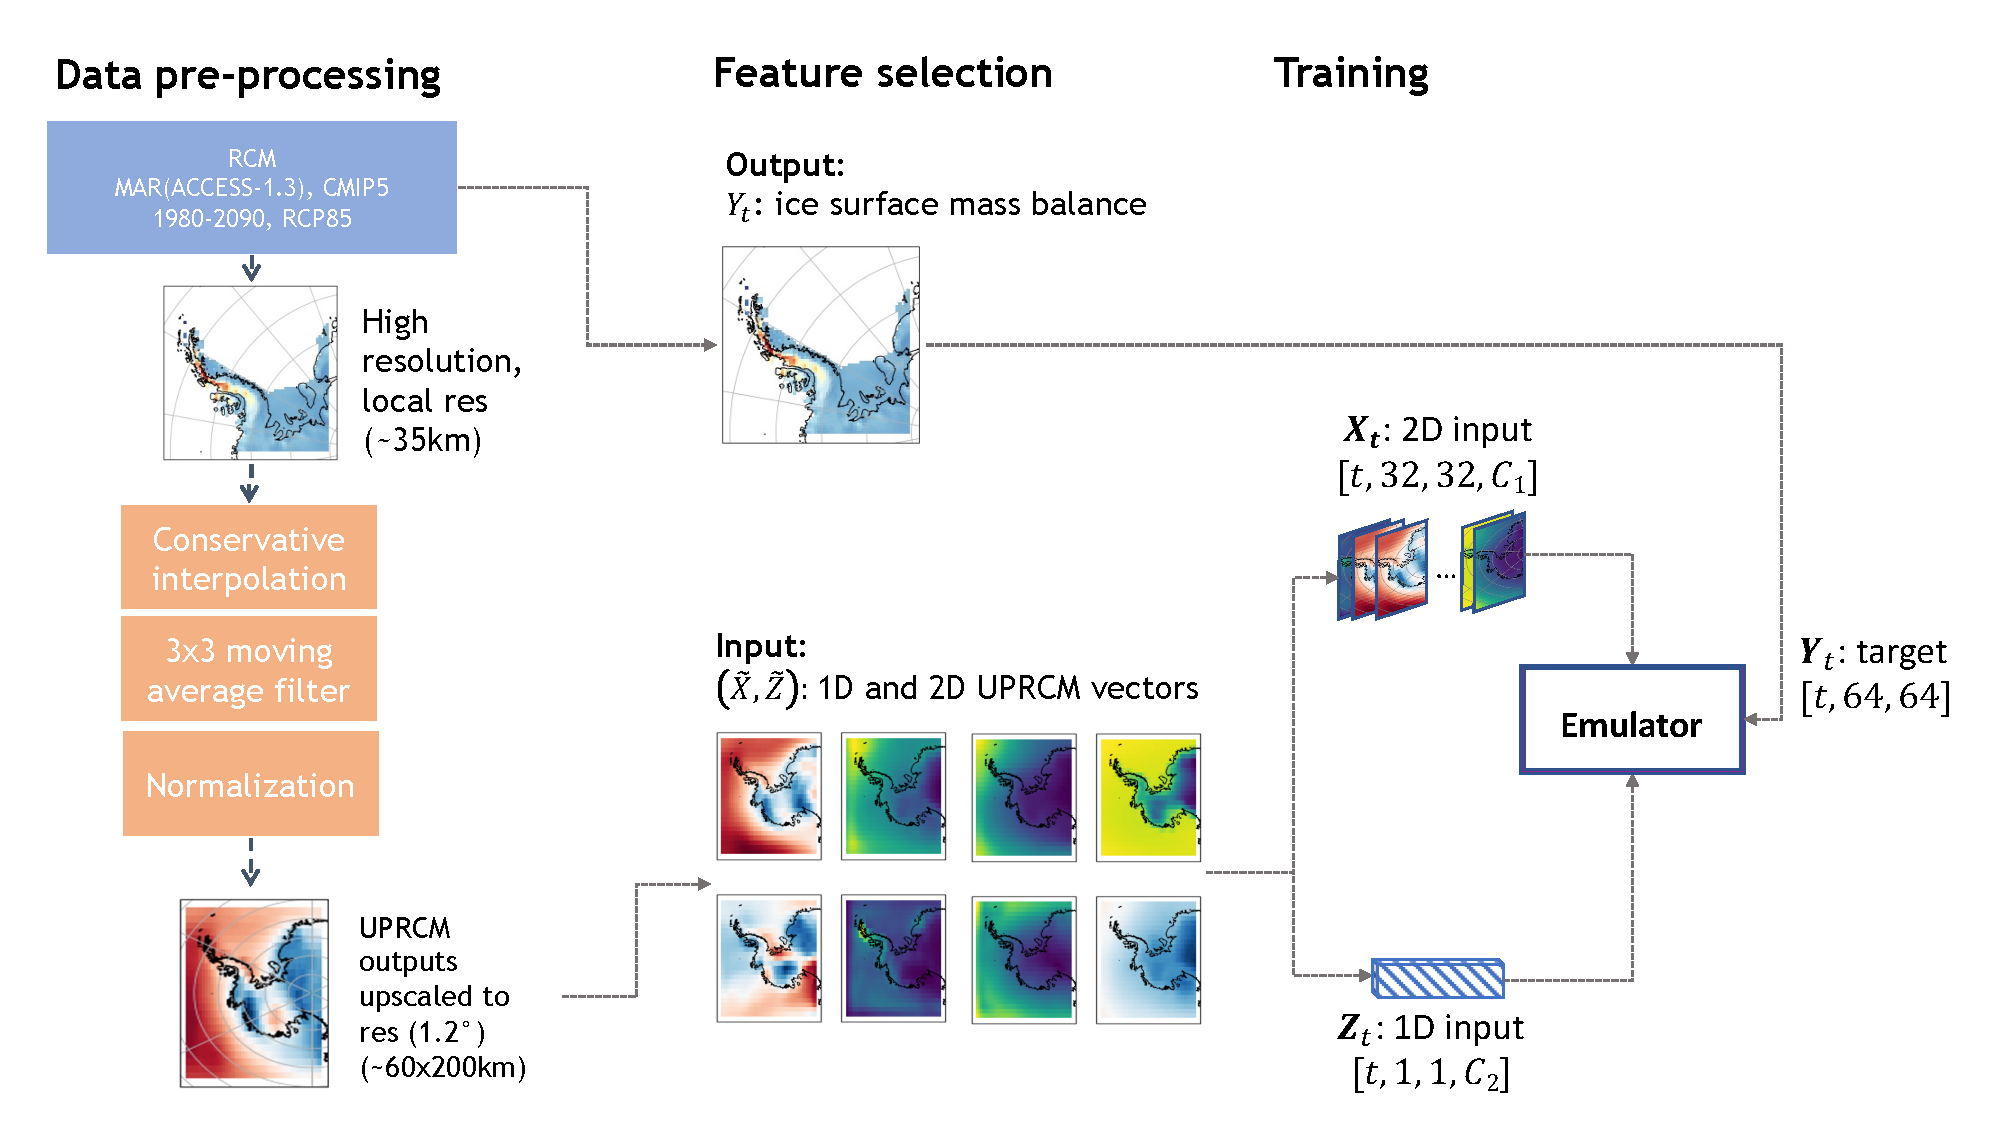
\includegraphics[width=\columnwidth]{images/data-flow.pdf}
  \caption []{\small RCM data flow to create UPRCM data.}
  \vspace{-3mm}
  \label{fig:training-data-flow}
\end{figure}



\end{document}